%!TEX TS-program = pdflatex
% Segal_Thesis.tex -- main dissertation file

\documentclass[12pt,oneside,letterpaper]{memoir}

\usepackage{tocloft}
\usepackage{titlesec}
\usepackage{setspace}
\usepackage{sidecap}
\usepackage{wrapfig}

\setlength{\parskip}{.1in}
\setlength{\intextsep}{20pt}
\setlength{\belowcaptionskip}{-12pt} 
%\setlength{\textfloatsep}{100pt} 
%\setlength{\fboxrule}{100}

\usepackage[top=1.25in, bottom=1in, left=1.25in, right=1in]{geometry}

\makeatletter
\renewcommand*\l@chapter{\@dottedtocline{1}{1.em}{2.4em}}
\renewcommand*\l@section{\@dottedtocline{1}{1.8em}{2.4em}}
\renewcommand*\l@appendix{\@dottedtocline{1}{1.em}{2.4em}}
\renewcommand*{\printchapternonum}{\chapnumfont \thechapter}
\makeatother 

% preamble.tex -- packages to include
%
% Wisconsin dissertation template
% Copyright (c) 2008 William C. Benton.  All rights reserved.
%
% This program can redistributed and/or modified under the terms
% of the LaTeX Project Public License Distributed from CTAN
% archives in directory macros/latex/base/lppl.txt; either
% version 1 of the License, or (at your option) any later version.
%
% This program includes other software that is licensed under the
% terms of the LPPL and the Perl Artistic License; see README for details.
%
% You, the user, still hold the copyright to any document you produce
% with this software (like your dissertation).

%% You should use natbib
\IfFileExists{natbib.sty}{%
\usepackage{natbib}%
\setcitestyle{square}
}{}

%% You probably need appendix, if you want appendices
\IfFileExists{appendix.sty}{%
\usepackage{appendix}%
}{}

%% the spacing in memoir is weird, you'll need to use this
\DisemulatePackage{setspace}
\usepackage[onehalfspacing]{setspace}

%% geometry package to help with margins on title page
\usepackage{geometry}

%% List setup; the ``hanglist`` environment will allow you to have
%% nicely-typeset enumerated lists (i.e. with the numbers hanging in
%% the margins).  You need at least version 2.1 of enumitem.sty.  If
%% you don't have enumitem installed at all, hanglist will just be an
%% alias for enumerate.
\IfFileExists{enumitem.sty}{%
\usepackage[loadonly]{enumitem}[2007/06/30]%
\newlist{hanglist}{enumerate}{1}% 
\setlist[hanglist]{label=\arabic*.}%
\setlist[hanglist,1]{leftmargin=0pt}%
}{%
\newenvironment{hanglist}{\begin{enumerate}}{\end{enumerate}}%
}

%% Comment out any of these that you don't want
\usepackage{amssymb}
\usepackage{amsmath}
\usepackage{amsthm}
%\usepackage{theorem}
\usepackage{hyperref}

\IfFileExists{mathpartir.sty}{%
\usepackage{mathpartir}%
}{}

%%%%% LISTINGS package and setup
\IfFileExists{listings.sty}{%
\usepackage{listings}%
}{}



%% Get rid of ugly borders around PDF hyperlinks (e.g. for cross-references, bib entries, or URLs)
\hypersetup{pdfborder = 0 0 0}

%% You want microtype.
\IfFileExists{microtype.sty}{%
\usepackage[protrusion=true,expansion=true]{microtype}%
}{}

%\pagestyle{thesisdraft}

% Surround parts of graphics with box
\usepackage{boxedminipage}

%% booktabs (thx to Nate Rosenblum for bringing this beautiful package
%% to my attention)
\IfFileExists{booktabs.sty}{%
\usepackage{booktabs}%
}{}

% This is now the recommended way for checking for PDFLaTeX:
\usepackage{ifpdf}

%% Avoid ugly "Type 3" fonts
\usepackage{lmodern}
\usepackage[LY1]{fontenc}

%% Substitute your favorite serif and sans fonts here....
\IfFileExists{tgpagella.sty}{%
% TeX Gyre pagella, like Palatino
\usepackage{tgpagella}%
}{}

\usepackage[LY1]{eulervm}

\usepackage[pdftex]{graphicx}

\usepackage{makeidx}
\makeindex

{\theoremstyle{plain}
\newtheorem{thm}{Theorem}[chapter]
\newtheorem{cor}[thm]{Corollary}
\newtheorem{define}[thm]{Definition}
\newtheorem{exmpl}[thm]{Example}
}
{\theoremstyle{remark}
\newtheorem{rmk}[thm]{Remark}
}

\newtheoremstyle{customsty1}
{3pt}%
{3pt}%
{}% --- body font
{}% --- indent amount
{\bfseries}% --- Theorem head font
{:}% --- Punctuation after head
{.5em}% --- space after head
{}% --- theorem head spec (can be left empty, meaning 'normal')

% Define 'newtheorems' that use ``customsty1''
{\theoremstyle{customsty1} 
}


%%% NB: the ``deposit'' chapter- and page- styles should conform to UW
%%% requirements.  If you are producing a pretty version of your
%%% dissertation for web use later, you will certainly want to make
%%% your own chapter and page styles.

\makechapterstyle{deposit}{%
  \renewcommand{\chapterheadstart}{}
  \renewcommand{\printchaptername}{}
  \renewcommand{\chapternamenum}{}
  \renewcommand{\printchapternum}{\parbox{2em}{\LARGE\textbf\thechapter{}} }
  \renewcommand{\afterchapternum}{}
  \renewcommand{\printchaptertitle}[1]{%
  \raisebox{-.6ex}{\raggedright\LARGE\textbf{##1}}}
  \renewcommand{\afterchaptertitle}{%
   \noindent\rule{\textwidth}{0.45mm} \vskip\onelineskip}
}

\makepagestyle{deposit}
 
\makeatletter
 
\renewcommand{\chaptermark}[1]{\markboth{#1}{}}
\renewcommand{\sectionmark}[1]{\markboth{#1}{}}
 
\makeevenfoot{deposit}{}{}{}
\makeoddfoot{deposit}{}{}{}
\makeevenhead{deposit}{\thepage}{}{}
\makeoddhead{deposit}{}{}{\thepage}
\makeatother

%%% set up page numbering for chapter pages to satisfy UW requirements
%%% NB: You will want to delete until the ``SNIP'' mark if you are
%%% making a ``nice'' copy
\copypagestyle{chapter}{plain}
\makeoddfoot{chapter}{}{}{}
\makeevenhead{chapter}{\thepage}{}{}
\makeoddhead{chapter}{}{}{\thepage}
%%% SNIP

%%% bib nonsense
\makeatletter
\newenvironment{wb-bib}[1]{%
  \chapter*{references}
\ifnobibintoc\else 
\phantomsection 
\addcontentsline{toc}{chapter}{References} 
\fi 
\prebibhook
  \begin{bibitemlist}{#1}}{\end{bibitemlist}\postbibhook}

\AtBeginDocument{%
  \@ifpackageloaded{natbib}{% natbib is loaded
    \addtodef{\endthebibliography}{}{\vskip-\lastskip\postbibhook}
    \@ifpackagewith{natbib}{sectionbib}{% with sectionbib option
      \renewcommand{\bibsection}{\@memb@bsec}}%
      {\renewcommand{\bibsection}{\@memb@bchap}}}%
  {}
  \@ifpackagewith{chapterbib}{sectionbib}{%
    \renewcommand{\sectionbib}[2]{}
    \renewcommand{\bibsection}{\@memb@bsec}}{}
}
\makeatother
\nouppercaseheads
% defs.tex -- wbepi environment for chapter epigraphs and other useful defs.
%
% Wisconsin dissertation template
% Copyright (c) 2008 William C. Benton.  All rights reserved.
%
% This program can redistributed and/or modified under the terms
% of the LaTeX Project Public License Distributed from CTAN
% archives in directory macros/latex/base/lppl.txt; either
% version 1 of the License, or (at your option) any later version.
%
% This program includes other software that is licensed under the
% terms of the LPPL and the Perl Artistic License; see README for details.
%
% You, the user, still hold the copyright to any document you produce
% with this software (like your dissertation).


%% put lstnewenvironment declarations here, if you're using listings

%% end lstnewenvironment declarations

%% I put convenience definitions that will go in several chapters here

%%%%% begin convenience definitions

\makeatletter
\newcommand{\wb@episource}{}
\newenvironment{wbepi}[1]{\begin{quote}\renewcommand{\wb@episource}{#1}\itshape}{\par\upshape \raggedleft --- \textbf{\wb@episource}\\ \end{quote}}
\makeatother

%%%%% SVN
\IfFileExists{svn-multi.sty}{%
\usepackage{svn-multi}%
%%% Uncomment the second one and comment out the first one if you want
%%% to include subversion revision information in each file.
\newcommand{\vcinfo}{}%
%\newcommand{\vcinfo}{\begin{centering}\fbox{\fbox{\parbox{5in}{Author: \svnauthor\\Revision: \svnfilerev\\Last changed on: \svnfiledate\\URL: \svnkw{HeadURL}}}}\\[1em]\end{centering}}%
}{%
\newcommand{\svnidlong}[4]{}%
\newcommand{\svnfilerev}{}%
\newcommand{\svnauthor}{}%
\newcommand{\svnfiledate}{}%
\newcommand{\svnkw}{}%
\newcommand{\vcinfo}{}%
}

%%%%% end convenience definitions

% thesisdefs.tex

% This is mostly adapted from withesis.cls.  The original copyright
% notice for withesis.cls follows, preceded by two percent signs (%%):

%% withesis.cls
%% LaTeX Style file for the University of Wisconsin-Madison Thesis Format
%% Adapted from the Purdue University Thesis Format
%% Originally by Dave Kraynie
%% Edits by Darrell McCauley
%% Adapted to UW-Madison format by Eric Benedict  (Noted with <EB>)
%% Updated to LaTeX2e by Eric Benedict 24 July 00
%% 
%%=============================================================================
%% Licensed under the Perl Artistic License.
%% see: http://www.ctan.org/tex-archive/help/Catalogue/licenses.artistic.html
%% for more info...
%%=============================================================================

% withesis.cls is available from CTAN.  The modifications to this file
% are also licensed under the Perl Artistic License.

% --wb, 2008

\makeatletter

\newcounter {tocpage}
\newcounter {lofpage}
\newcounter {lotpage}
\newcounter {listofheading}

\newcommand\@thesistitlemedskip{0.25in}
\newcommand\@thesistitlebigskip{0.6in}
\newcommand{\degree}[1]{\gdef\@degree{#1}}
\newcommand{\project}{\gdef\@doctype{A masters project report}}
\newcommand{\prelim}{\gdef\@doctype{A preliminary report}}
\newcommand{\thesis}{\gdef\@doctype{A thesis}}
\newcommand{\dissertation}{\gdef\@doctype{A dissertation}}
\newcommand{\department}[1]{\gdef\@department{(#1)}}
\newcommand{\oralexamdate}[1]{\gdef\@oralexamdate{#1}} 
\newcommand{\committeeone}[1]{\gdef\@committeeone{#1}}
\newcommand{\committeetwo}[1]{\gdef\@committeetwo{#1}}
\newcommand{\committeethree}[1]{\gdef\@committeethree{#1}}
\newcommand{\committeefour}[1]{\gdef\@committeefour{#1}}
\newcommand{\committeefive}[1]{\gdef\@committeefive{#1}}
\newcommand{\committeesix}[1]{\gdef\@committeesix{#1}}
\newcommand{\committeeseven}[1]{\gdef\@committeeseven{#1}}

\newenvironment{titlepage}
 {\@restonecolfalse\if@twocolumn\@restonecoltrue\onecolumn
  \else \newpage \fi \thispagestyle{empty}
% \c@page\z@ -- deleted: count title page in thesis
}{\if@restonecol\twocolumn \else \newpage \fi}

\gdef\@degree{Bachelor of Science}    %Default is PhD
\gdef\@doctype{A thesis}         %Default is dissertation

\gdef\@department{(Electrical Engineering)} % Default is Electical Engineering
\gdef\@oralexamdate{}
\gdef\@committeeone{}
\gdef\@committeetwo{}
\gdef\@committeethree{}
\gdef\@committeefour{}
\gdef\@committeefive{}
\gdef\@committeesix{}
\gdef\@committeeseven{}



\renewcommand{\maketitle}{%
  \begin{titlepage}
  \begin{vplace}%[0.7]
%-----------------------------------------------------------------------------
% -- The thesis office doesn't like thanks on title page.  Put it in
% -- the acknowledgments.  This is here so you don't have to change
% -- your titlepage when converting from report style. -> from Purdue, but I
%        left it here since it seems compatible with UW-Madison, Eric
%-----------------------------------------------------------------------------
    \def\thanks##1{\typeout{Warning: `thanks' deleted from thesis titlepage.}}
    \let\footnotesize\small \let\footnoterule\relax \setcounter{page}{1}
 %sets new margins for title page so that committee members can be placed there

   % \vspace*{0.1in}
    \begin{center}
      {\textbf{\expandafter\expandafter{\@title}}} \\[\@thesistitlebigskip]
       by \\[\@thesistitlemedskip]
      \@author \\[\@thesistitlebigskip]
      \@doctype\ submitted in partial fulfillment of \\
      the requirements for the degree of\\[\@thesistitlebigskip]
      \@degree \\[\@thesistitlemedskip]
      \@department \\[\@thesistitlebigskip]
      at the \\[\@thesistitlebigskip]
      UNIVERSITY OF WISCONSIN--MADISON\\[\@thesistitlebigskip]
      \@date \\[\@thesistitlebigskip]
    \end{center}
% section added by Steven Baumgart on 3/2012
% adds committee list to the title page
% add or delete committee members as you need to, these are defined in the dissertation.tex document 
% comment out other things as you need to as well. - SB

%\noindent Date of final oral examination: \@oralexamdate \hspace*{\fill} \\[\@thesistitlemedskip]
%\noindent The dissertation is approved by the following members of the Final Oral Committee:\\*
%\indent \@committeeone\\*
%\indent \@committeetwo\\*
%\indent \@committeethree\\*
%\indent \@committeefour

  \end{vplace}
  \end{titlepage}


  \setcounter{footnote}{0}
  \setcounter{page}{1} %title page is NOT counted
  \let\thanks\relax
  \let\maketitle\relax \let\degree\relax \let\project\relax \let\prelim\relax
  \let\department\relax
  \gdef\@thanks{}\gdef\@degree{}\gdef\@doctype{}
  \gdef\@department{}
  %\gdef\@author{}\gdef\@title{}
}


%=============================================================================
% ABSTRACT
%=============================================================================
% The abstract should begin with two single-spaced lines describing
% the author and title in a standard format.  After these lines comes
% the standard abstract.
%=============================================================================
\def\abstract{
  \section*{Abstract}
  \addcontentsline{toc}{chapter}{Abstract}
  \relax\markboth{Abstract}{Abstract}}
\def\endabstract{\par\newpage}


%=============================================================================
% UMI ABSTRACT
%=============================================================================
% The UMI abstract should begin with the author and title in a standard format.
% After the author comes the advisor and university. After these lines comes
% a bunch of double spaced text to make up the standard abstract.
% After the abstract, the advisor's approval signature follows.
% This page is not numbered and is delivered seperately to the thesis office.
%=============================================================================

\def\advisortitle#1{\gdef\@advisortitle{#1}}
\def\advisorname#1{\gdef\@advisorname{#1}}
\gdef\@advisortitle{Professor}
\gdef\@advisorname{Cheer E.\ Place}

\def\umiabstract{
             \thispagestyle{empty}
                  \addtocounter{page}{-1}
                \begin{center}
                  {\textbf{\expandafter\expandafter{\@title}}}\\
                  \vspace{12pt}
                  \@author \\
                  \vspace{12pt}
                  Under the supervision of \@advisortitle\ \@advisorname\\
                  At the University of Wisconsin-Madison
                \end{center}
}

\def\endumiabstract{\vfill \hfill\@advisorname\par\newpage}


%============================================================================
% VERBATIMFILE
%============================================================================
% \verbatimfile{<filename>}    for verbatim inclusion of a file
% - Note that the precise layout of line breaks in this file is important!
% - added the \singlespace - EB
%============================================================================
\def\verbatimfile#1{\begingroup \singlespace
                    \@verbatim \frenchspacing \@vobeyspaces
                    \input#1 \endgroup
}


%=============================================================================
% SEPARATOR Pages
%   Creates a blank page with a text centered horizontally and vertically.
%   The page is neither counted nor numbered.
%   These pages are required in the thesis format before sections such
%   as appendices, vita, bibliography, etc.
%=============================================================================
\def\separatorpage#1{
  \newpage
  \thispagestyle{empty}
  \addtocounter{page}{-1}
  \null
  \vfil\vfil
  \begin{center}
    {\textbf{#1}}
  \end{center}
  \vfil\vfil
  \newpage}


%=============================================================================
% COPYRIGHTPAGE
%=============================================================================
% The copyright must do the following:
% - start a new page with no number
% - place the copyright text centered at the bottom.
%=============================================================================
\def\copyrightpage{}


%=============================================================================
% GLOSSARY
%=============================================================================
% The glossary environment must do the following:
% - produce the table of contents entry for the glossary
% - start a new page with GLOSSARY centered two inches from the top
%=============================================================================
\def\glossary{
  \section*{GLOSSARY}
  \addcontentsline{toc}{section}{Glossary}}
\def\endglossary{\par\newpage}

%=============================================================================
% NOMENCLATURE
%=============================================================================
% The nomenclature environment must do the following:
% - produce the table of contents entry for the nomenclature section
% - start a new page with NOMENCLATURE centered two inches from the top
%=============================================================================
\def\nomenclature{}

%=============================================================================
% CONVENTIONS
%=============================================================================
% The conventions environment must do the following:
% - produce the table of contents entry for the nomenclature section
% - start a new page with CONVENTIONS centered two inches from the top
%=============================================================================
\def\conventions{}


%=============================================================================
% COLOPHON
%=============================================================================
% The colophon environment must do the following:
% - produce the table of contents entry for the nomenclature section
% - start a new page with COLOPHON centered two inches from the top
%=============================================================================
\def\colophon{\separatorpage{DISCARD THIS PAGE}
  \chapter*{Colophon}
  \addcontentsline{toc}{chapter}{Colophon}}
\def\endcolophon{\par\newpage}

%=============================================================================
% LIST OF SYMBOLS
%=============================================================================
% The list of symbols environment must do the following:
% - produce the table of contents entry for the list of symbols section
% - start a new page with LIST OF SYMBOLS centered two inches from the top
%=============================================================================
\def\listofsymbols{\separatorpage{DISCARD THIS PAGE}
  \eject
  \chapter*{LIST OF SYMBOLS}
  \addcontentsline{toc}{chapter}{LIST OF SYMBOLS}}
\def\endlistofsymbols{\par\newpage}

%=============================================================================
% VITA
%=============================================================================
% The vita environment must do the following:
% - produce a separator page with the word vita centered
% - produce the table of contents entry for the vita
% - start a new page with VITA centered two inches from the top
%=============================================================================
\def\vita{
%  \separatorpage{VITA}         % UW doesn't require this EB
  \chapter*{VITA}
  \addcontentsline{toc}{chapter}{VITA}}
\def\endvita{\par\newpage}

%=============================================================================
% ACKNOWLEDGMENTS
%=============================================================================
% The acknowledgments environment must do the following:
% - start a new page with ACKNOWLEDGMENTS centered two inches from the top
%=============================================================================
\def\acks{
  \section*{Acknowledgments}
}
\def\endacks{\par\newpage}

%=============================================================================
% DEDICATION
%=============================================================================
% The dedication environment must do the following:
% - start a new page
% - center the text vertically
% - include the text in a center environment
%=============================================================================
\def\dedication{
  \newpage
  \null\vfil
  \begin{center}}
\def\enddedication{\end{center}\par\vfil\newpage}

%=============================================================================
% DATE
%=============================================================================
%\def\today{\ifcase\month\or
  %January\or February\or March\or April\or May\or June\or
  %July\or August\or September\or October\or November\or December\fi
  %\space\number\day, \number\year}
\newcount\@testday
\def\today{\@testday=\day
  \ifnum\@testday>30 \advance\@testday by -30
  \else\ifnum\@testday>20 \advance\@testday by -20
  \fi\fi
  \number\day\ \
  \ifcase\month\or
    January \or February \or March \or April \or May \or June \or
    July \or August \or September \or October \or November \or December
    \fi\ \number\year
}


%  Single counter for theorems and theorem-like environments:
\newtheorem{theorem}{Theorem}[chapter]
\newtheorem{assertion}[theorem]{Assertion}
\newtheorem{claim}[theorem]{Claim}
\newtheorem{conjecture}[theorem]{Conjecture}
\newtheorem{corollary}[theorem]{Corollary}
\newtheorem{definition}[theorem]{Definition}
\newtheorem{example}[theorem]{Example}
\newtheorem{figger}[theorem]{Figure}
\newtheorem{lemma}[theorem]{Lemma}
\newtheorem{prop}[theorem]{Proposition}
\newtheorem{remark}[theorem]{Remark}

%=============================================================================
% BIBLIOGRAPHY
%=============================================================================
% The thebibliography environment executes the following commands:
%
%  o start a new 'chapter' with BIBLIOGRAPHY as the heading
%  o produce a separator page for the bibliography
%
%  \def\newblock{\hskip .11em plus .33em minus -.07em} --
%      Defines the `closed' format, where the blocks (major units of
%      information) of an entry run together.
%
%  \sloppy  -- Used because it's rather hard to do line breaks in
%      bibliographies,
%
%  \sfcode`\.=1000\relax --
%      Causes a `.' (period) not to produce an end-of-sentence space.
%=============================================================================
% \altbibtitle
%   The default title for the References chapter is ``LIST OF REFERENCES''
%   Since some people prefer ``BIBLIOGRAPHY'', the command
%   \altbibtitle has been added to change the chapter title.
%   This command does nothing more than change REFERENCES to BIBLIOGRAPHY
%============================================================================
\def\@bibchaptitle{\textbf{References}}
\def\altbibtitle{\def\@bibchaptitle{Bibliography}}
\def\thebibliography#1{
  %\separatorpage{\@bibchaptitle}
  \global\@bibpresenttrue
  \chapter[\textbf{References}]{References}
  \vspace{0.375in}    % added to match 4 line requirement
  \interlinepenalty=10000 % added to prevent breaking of bib entries
  \singlespace\list
  {[\arabic{enumi}]}{\settowidth\labelwidth{[#1]}\leftmargin\labelwidth
    \advance\leftmargin\labelsep \usecounter{enumi}}
  \def\newblock{\hskip .11em plus .33em minus -.07em}
  \sloppy
  \sfcode`\.=1000\relax}
\let\endthebibliography=\endlist



\makeatother


\svnidlong{$LastChangedBy$}{$LastChangedRevision$}{$LastChangedDate$}{$HeadURL: http://freevariable.com/dissertation/branches/diss-template/dissertation.tex $} 

\clearpage\pagenumbering{roman}  % This makes the page numbers Roman (i, ii, etc)

\title{AHAB \\ --- OR --- \\ The Hunt for Automated Shock Timing}
\author{Daniel J. Segal}
\department{Engineering Physics}

\oralexamdate{8/22/14}
\date{2014}

\tolerance=1
\emergencystretch=\maxdimen
\hyphenpenalty=10000
\hbadness=10000


\begin{document}

	\addtocontents{toc}{\protect\setstretch{1.8}}
	\captionnamefont{\bfseries}
	\captiontitlefont{\bfseries}

	\newgeometry{left=1.25in,right=1.25in,bottom=1.25in,top=1.25in}
	\maketitle
	\restoregeometry %sets the margins back to normal

	\svnidlong{$LastChangedBy$}{$LastChangedRevision$}{$LastChangedDate$}{$HeadURL: http://freevariable.com/dissertation/branches/diss-template/frontmatter/frontmatter.tex $}
\vcinfo{}

%%% SOME OF THIS CODE IS ADAPTED FROM THE VENERABLE withesis.cls


%% BEGIN PAGESTYLE

%%% You can pick a pagestyle if you want; see the memoir class
%%% documentation for more info.  The default ``deposit'' option meets
%%% the UW thesis typesetting requirements but is probably
%%% unsatisfactory for making a version of your dissertation that
%%% won't be deposited to the graduate school (e.g. for web or a nice
%%% printed copy)

\chapterstyle{deposit}
\pagestyle{deposit}

\advisorname{Gregory Moses}
\advisortitle{Professor}

% ACKNOWLEDGMENTS
%\begin{acks}
%\input{frontmatter/acks}
%\end{acks}

% CONTENTS, TABLES, FIGURES
\renewcommand{\printtoctitle}[1]{\section*{#1}}
\renewcommand{\printloftitle}[1]{\section*{#1}}
\renewcommand{\printlottitle}[1]{\section*{#1}}

\renewcommand{\tocmark}{}
\renewcommand{\lofmark}{}
\renewcommand{\lotmark}{}

\renewcommand{\tocheadstart}{}
\renewcommand{\lofheadstart}{}
\renewcommand{\lotheadstart}{}

\renewcommand{\aftertoctitle}{}
\renewcommand{\afterloftitle}{}
\renewcommand{\afterlottitle}{}

\renewcommand{\cftchapterfont}{\normalfont} 
\renewcommand{\cftsectionfont}{\itshape} 
\renewcommand{\cftchapterpagefont}{\normalfont} 
\renewcommand{\cftchapterpresnum}{\bfseries} 
\renewcommand{\cftchapterleader}{} 
\renewcommand{\cftsectionleader}{} 

%\renewcommand{\cftchapafterpnum}{\addvspace{150pt}}
%\renewcommand{\cftsecafterpnum}{\addvspace{150pt}}
% \captionnamefont{\small\sffamily} 
% \captiontitlefont{\small\sffamily} 

% \renewcommand{\contentsname}{contents}
% \renewcommand{\listfigurename}{list of figures}
% \renewcommand{\listtablename}{list of tables}

\addtocontents{toc}{\protect\addvspace{12pt}}%

\tableofcontents

\makeatletter \renewcommand{\@dotsep}{4.5} \makeatother

\clearpage
%\listoftables

%\vspace{2cm}

\listoffigures

\clearpage
% NOMENCLATURE
% \begin{conventions}
% % \begin{description}
% % \item{\makebox[0.75in][l]{term}
% %        \parbox[t]{5in}{definition\\}}
% % \end{description}
% \input{conventions}
% \end{conventions}


% ABSTRACT

\begin{abstract}
  
\setlength{\parindent}{0cm}

Shock Ignition is a form of ignition for Inertial Confinement Fusion, which promises gains that are nearly an order of magnitude larger than NIF baseline values.  Although a relatively new scheme, Shock Ignition has received a considerable amount of research attention due to its ability to be applied to currently implemented technology.

A major component of Shock Ignition is computational modeling. One fundamental problem involved in it is the timing of laser-induced shocks, so that they coalesce at the same radius of their target.  AHAB -- or Automated High-throughput computing Achieved with Batch processing -- was designed to help with this timing process.  It has since grown to be capable of conducting parameter sweeps for a large set of optimization studies and debugging processes.

\setlength{\parindent}{\default}

\addtocontents{toc}{\protect\vspace{20pt}}
\end{abstract}

\clearpage\pagenumbering{arabic}

%%% END STUFF TAKEN FROM WITHESIS EXAMPLE FILE

	%\frontmatter

	%\include{mainmatter/mainmatter}
	%\mainmatter

	\begingroup

		\midsloppy
		\let\clearpage\relax
		\setlength{\parindent}{0cm}
		%\let\uppercase\relax

\chapter[\textbf{Introducing Shock Ignition}]{Introducing Shock Ignition}
  %\addcontentsline{toc}{chapter}{Glassary}

In today`s economic climate, energy is a precious commodity; it is therefore a leading factor in the design of most engineering budgets.  In an effort to change this paradigm, many societies have attempted to stray away from using traditional fossil fuels and move towards other forms of large-scale energy production.  

One potential source for this energy production is nuclear fusion, the same process that powers the sun. The reason this form of energy production has not been realized in a reactor setting, though, is because a feasible reactor would need to confine an extremely hot, dense plasma.  Because these terrestrial plasmas cannot take advantage of the large gravitational forces present in the sun, other schemes for their confinement are needed.

%The reason this form of energy production has not been realized in a reactor setting, though, is because it needs to confine its extremely hot, dense plasma.  Because these terrestrial plasmas cannot take advantage of the large gravitational forces present in the sun, other schemes for their confinement are needed.

  \section{Confining a Plasma using its own Inertia}
  %\addcontentsline{toc}{section}{Glossary}

Inertial confinement fusion (ICF) is a method for achieving fusion that utilizes a plasma`s own inertia as a form of confinement.  In it, a spherical array of high-intensity lasers deposits energy onto a small plastic target filled with Hydrogen isotopes, see Fig.\,\ref{fig:laser}.  The energy deposited by these lasers serves to both heat and compress the target, causing its Hydrogen fuel source to reach the temperatures and the pressures needed for ignition, or the initiation of a sustained fusion chain reaction \citep{mosesBook}.  

\begin{SCfigure}[][h!]	
	\centering
	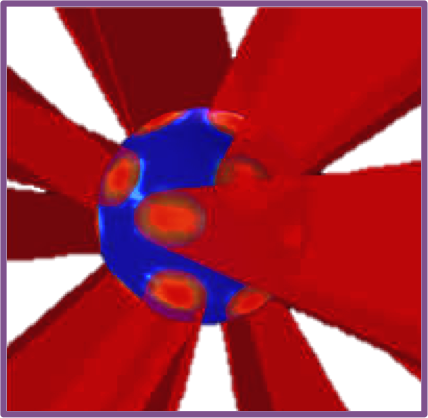
\includegraphics[scale=.95]{graphics/laserFusion.png}
	\caption[Inertial Confinement Fusion]{ \\ Inertial Confinement Fusion \\ \captiontitlefinal{\textmd{is sometimes referred to as laser-driven fusion because it involves shooting a millimeter-sized target with an array of lasers. This image captures how the areal projections of the lasers impact the spherical symmetry of the problem \citep{aNewShock}. } } }
	\label{fig:laser}
\end{SCfigure}

After ignition, the fuel source continues to burn until a dismantling shockwave - originating at the center - has a chance to propagate outwards.  Once this shockwave reaches the target`s shell, it ruptures the surrounding plasma envelope and causes the target to explode.  The optimization problem at hand, then, is to maximize the number of fusion reactions that occur in the nanoseconds-length time window between the target`s ignition and subsequent explosion.

In order to develop a working inertial fusion reactor, though, many implementation decisions and technologies still need to be made.  Several research facilities exist to investigate such issues, most notably the one at the National Ignition Facility in Livermore, California (Fig.\,\ref{fig:nif}).  At these facilities, one issue that gets a considerable amount of research attention is the type of ignition.  

\begin{SCfigure}[][h!]	
	\centering
	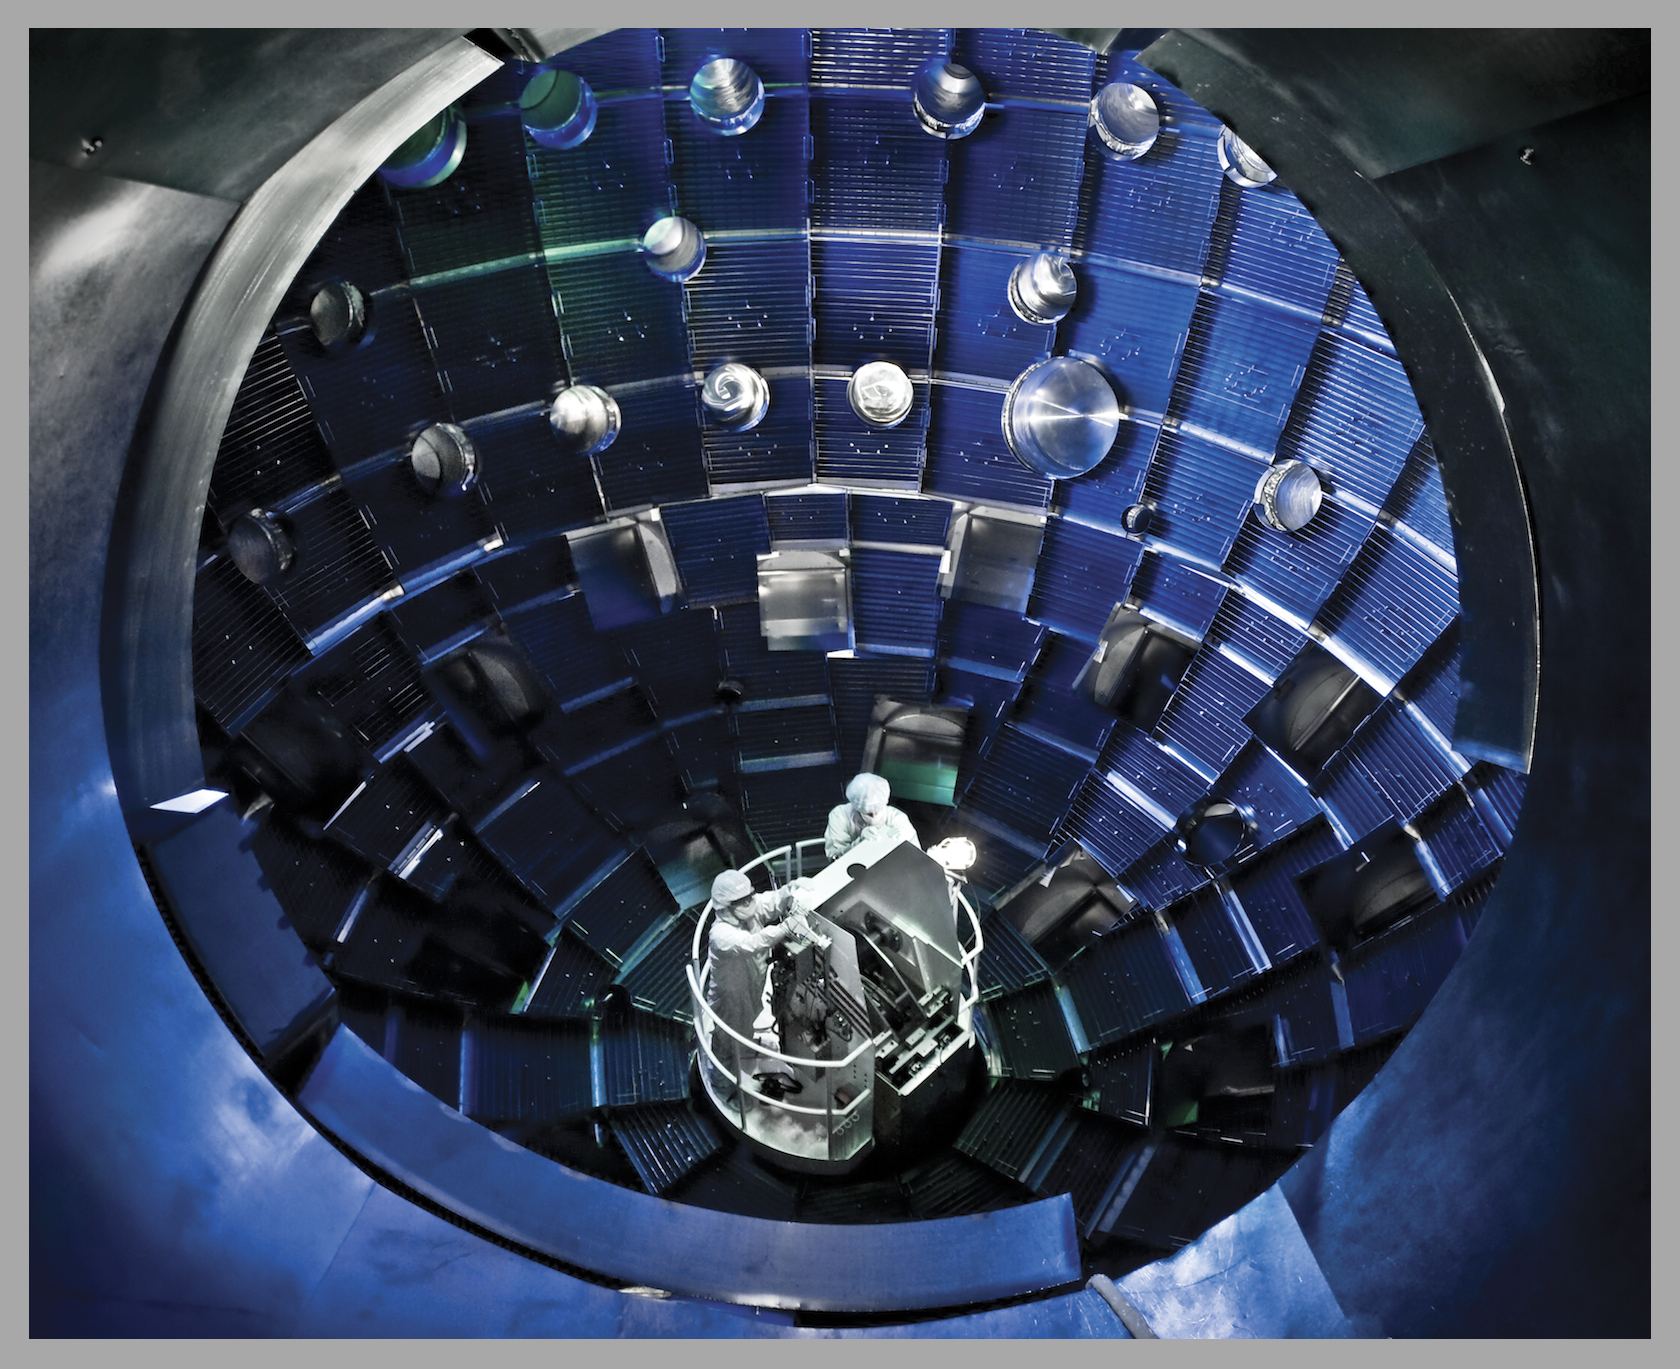
\includegraphics[scale=.4]{graphics/nif.jpg} 
	\caption[The National Ignition Facility]{ \\ The National Ignition Facility \\ \captiontitlefinal{\textmd{houses the world's largest laser array.  Inside the holes of the spherical chamber are nearly two-hundred lasers.  At roughly ten meters, the chamber itself is four orders of magnitude larger than the plastic targets it ignites. } } }
	\label{fig:nif}
\end{SCfigure}

Currently, the two most common types of ignition are direct drive and indirect drive.  In direct drive ignition, the laser array focuses directly on a target; while in indirect drive ignition, the laser array focuses on a gold shell surrounding the target that then deposits X-rays onto the target.  Although these two types of ignition are the most common, others exist: one prospective type being shock ignition \citep{summaryPaper}. 

\section{Achieving Ignition with Aligned Shock Fronts}

Shock ignition gets its name from how it achieves ignition: by timing shockwaves so that they add constructively at the center of a fuel target. The reason these shockwaves are able to reach a specific location simultaneously is because of their different speeds.  

In shock ignition, shockwaves are produced asynchronously by fluctuations in laser power.  Therefore, to have each shockwave coalesce at a certain radius later on, faster and faster wave speeds are needed for each successive shock.  Because these wave speeds are positively correlated to laser power, shock convergence can be achieved with a laser profile of individual pulses that increase in power. This then transforms the problem of aligning shockwaves into one of tuning a laser array's power versus time profile \citep{terryThesis}.  

This problem of constructing a laser array's power vs.\ time profile is the fundamental difference between shock ignition and other leading ignition schemes.  In conventional schemes for ignition, laser array profiles are designed to couple the compression stage and the ignition stage of the target, while in shock ignition, the profiles are designed to decouple them \citep{perkinsPaper}. 

As shown in Fig.\,\ref{fig:laserProfile}, this decoupling is accomplished by dividing the main laser pulse, which accounts for most of the energy consumption, into two separate pulses: a compression pulse and an igniter pulse.  The compression pulse, which is a relatively long, weak pulse, is designed to heat and to compress the target.  While, the igniter pulse, which is a relatively quick, high intensity burst, is designed to actually cause the target to ignite.  This decoupling of the two pulses leads to shock ignition having several unique characteristics when compared to other forms of ignition.  

\sidecaptionvpos{figure}{c}

\begin{SCfigure}[][h!]	
	\centering
	\caption[Laser Power versus Time Profiles]{ \\ Laser Power vs. Time \\ Profiles for Shock Ignition \\ and Direct Drive Ignition. \\ \captiontitlefinal{\textmd{Shock ignition differs from Direct Drive ignition in the way its laser profile is constructed.  Shock ignition separates what would be the main pulse into two pulses, which consequently decouples the target's compression stage and its ignition stage \citep{perkinsPaper}. } } }
	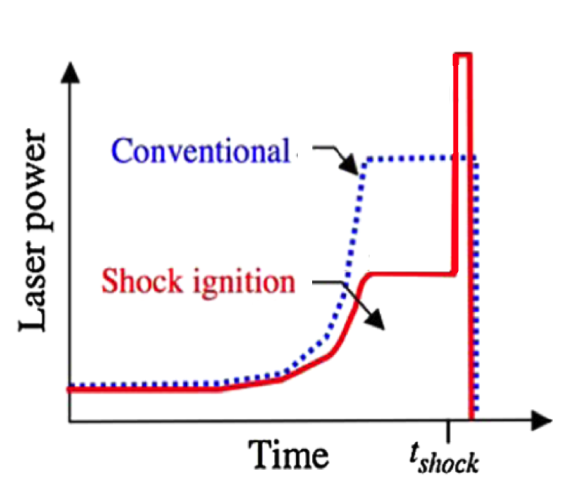
\includegraphics[scale=1]{graphics/laserProfile.png} 
	\label{fig:laserProfile}
\end{SCfigure}

\pagebreak

The major advantage shock ignition has over other competing ignition schemes is that its targets prospectively produce higher net gains, see Fig.\,\ref{fig:gainCurve}.  Here, a gain is defined as the ratio of fusion energy produced to the driver energy incident on the target, where a higher gain would correlate to a higher return of energy \citep{mosesBook}.  

\begin{SCfigure}[][h!]	
	\centering
	\caption[Gain Curve for Shock Ignition]{ \\ Gain as a function of \\ Laser Energy for Shock Ignition.   \\ \captiontitlefinal{\textmd{Early 1-D simulations show that the gains from shock ignition targets not only exceed the NIF baseline requirements, but also surpass those of candidate targets for both direct drive ignition (DD) and polar direct drive ignition (PDD) by nearly an order of magnitude \citep{perkinsPaper}. } } }
	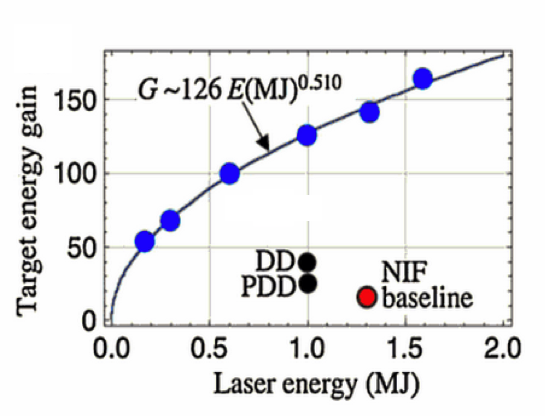
\includegraphics[scale=0.95]{graphics/gainCurve.png} 
	\label{fig:gainCurve}
\end{SCfigure}

\sidecaptionvpos{figure}{b}

Shock ignition is capable of achieving these gains because its targets have longer burn times, a consequence of the relatively low implosion velocities and thick instability-resilient shells inherent to the process \citep{perkinsPaper}.  A corollary of these high gains is that a feasible shock ignition reactor could produce the same amount of energy as any other potential inertial fusion reactor with a much weaker, and thus a much cheaper, laser \citep{summaryPaper}.  

In order for shock ignition to actually achieve these gains, though, its laser array's power versus time profile has to be constructed properly.  This construction process entails combining several laser pulses together in a very specific configuration.  Here a laser pulse is a section of the power versus time profile that has some definite shape, such as a horizontal line or a Gaussian curve.  

In addition to being constructed properly, a laser profile needs to be constructed efficiently.  There are several reasons for this.  First, because time at inertial fusion research facilities is expensive, many simulations are needed to justify every set of experiments.  Second, because there are so many research branches, e.g. target design and polar drive, the number of simulations needs to be minimized.

		%\let\uppercase\relax

\vspace{24pt}

\chapter[\textbf{Constructing a Laser Profile}]{Constructing a Laser Profile}

Shock ignition involves aligning shockwaves so that they coalesce at the center of a target.  Because these shockwaves are the result of fluctuations in laser power, the laser profile containing these fluctuations must be constructed with a thorough and robust algorithm.  

As shown in Fig.\,\ref{fig:profConst}, there are six different laser pulses that constitute a shock ignition laser profile: a picket pulse, three pedestal pulses, a compression pulse, and an igniter pulse.  In terms of comparing shock ignition to other forms of ignition, the compression pulse and igniter pulse are the major differences, when it comes to power considerations.

\sidecaptionvpos{figure}{c}

\begin{SCfigure}[][h!]	
	\centering
	\caption[A Laser Power versus Time Profile]{ An Example Laser \\ Power versus Time Profile. \\ \captiontitlefinal{\textmd{A laser power versus time profile for shock ignition has six individual pulses.  It has: an initial picket pulse to develop a plasma envelope surrounding the target, three pedestal pulses to increase the target's density, a compression pulse, and a final igniter pulse \citep{terryThesis}. } } }
	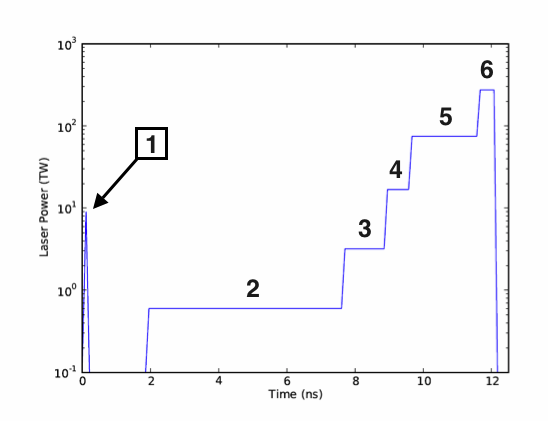
\includegraphics[scale=0.9]{graphics/profConst.png} 
	\label{fig:profConst}
\end{SCfigure}

\sidecaptionvpos{figure}{b}

  \section{Imposing a Picket Pulse}

The picket pulse`s main goal is to set the initial conditions of the simulation correctly.  Before the target is irradiated, it is a cryogenic piece of Hydrogen enclosed by a plastic shell.  The picket pulse is used to develop a plasma envelope surrounding the target.

This plasma envelope is useful for several reasons.  First, it increases the uniformity of laser absorption, which increases the spherical symmetry of the problem \citep{terryPaper}.  Second, it decreases the rate of instability growth on the shell`s surface, see Fig.\,\ref{fig:picketEffect}.  

\sidecaptionvpos{figure}{c}

\begin{SCfigure}[][h!]	
	\centering
	\caption[The Picket Pulse]{The Picket Pulse \\ \captiontitlefinal{\textmd{is designed to reduce the growth of Rayleigh-Taylor Instabilities (RTIs).  In this figure, the simulated RTI growth rate is taken as the linear growth rate in the 1.5 second window following the convergence of the three pedestal pulses at the ice-gas Hydrogen boundary for a wide range of mode numbers \citep{picketPaper}. } } }
	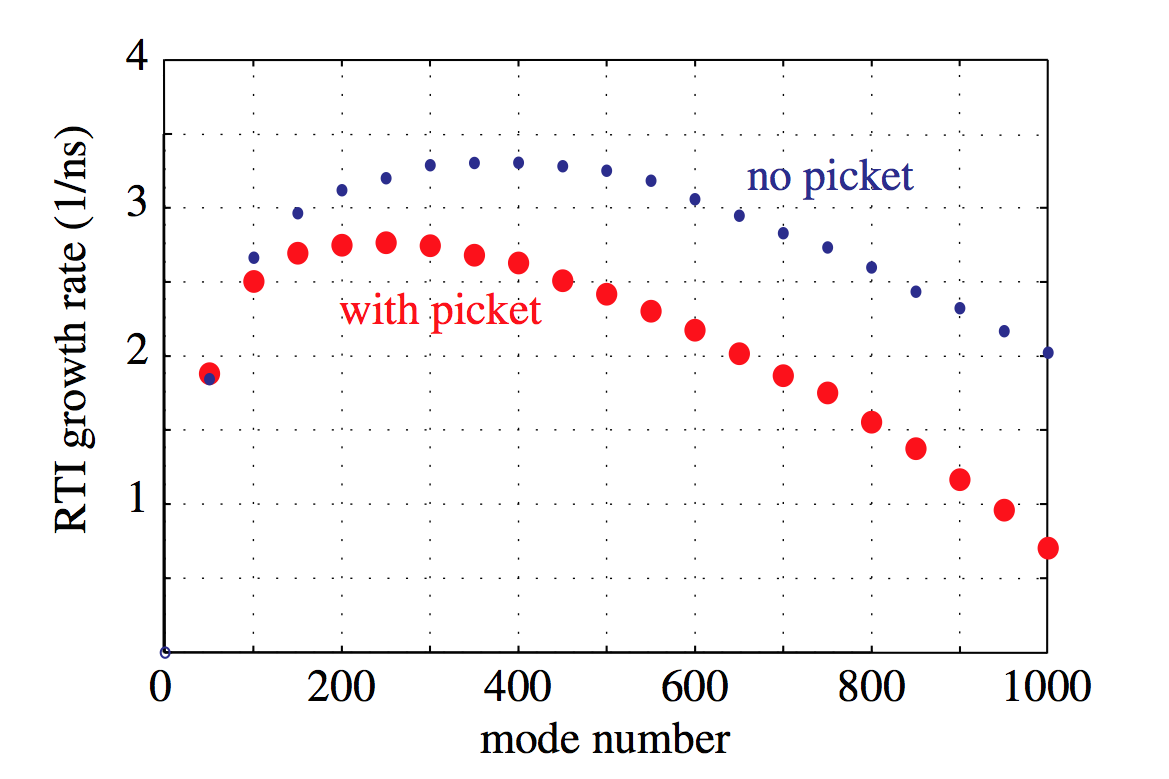
\includegraphics[width=0.55\textwidth]{graphics/picketEffect.png} 
	\label{fig:picketEffect}
\end{SCfigure}

\sidecaptionvpos{figure}{b}

  \section{Setting up Pedestal Pulses}
  \label{sec:pedestal}
The goal of the pedestal pulses is to increase the target`s fuel density by a factor of thirty, with a minimal amount of compression in the target. There are three pedestal pulses because each resulting shock is only theoretically capable of increasing the fuel density by a factor of four. Therefore, to achieve the sought after factor of thirty increase in fuel density, a minimum of three consecutive pulses are needed \citep{terryThesis}.  

To maximize the energy gain, the pedestal pulses need to be timed so that their resulting shockwaves arrive at the interface that exists between the outer Hydrogen ice shell and the inner Hydrogen gas region within fifty picoseconds of each other.  This interface is the optimum location for two reasons.  First, if the shockwaves were to pass each other within the Hydrogen ice region, they would cause unnecessary shock heating of the fuel.  Second, if the pulses were to meet inside the Hydrogen gas region, they would cause the fuel to decompress, which would be counter-productive to the process \citep{resultsVsSims}.

\section{Optimizing the Compression and Igniter Pulses}
\label{sec:mainPulses}
After the target`s density has increased by a factor of thirty, two more pulses are needed: the compression pulse and the igniter pulse.  Where constructing the picket pulse and the pedestal pulses required coalescing the resulting shockwaves at a single location, constructing the main pulses involves optimizing certain variables.  For the compression pulse, the maximized variable is the target`s density; for the igniter pulse, the maximized variable is the energy yield \citep{terryThesis}.

		%\let\uppercase\relax

\vspace{24pt}

\chapter[\textbf{Modeling Shock Ignition}]{Modeling Shock Ignition}

Before shock ignition experiments can be conducted at research facilities, such as the National Ignition Facility, the algorithm used for tuning the involved laser profiles needs to be both efficient and robust.  It needs to be efficient because each experiment involved in an actual tuning process requires more than a hundred simulations \citep{terryThesis}.  It needs to be robust because the output from the simulations needs to transfer to successfully timed experiments without too much calibration \citep{terryPaper}.  

In this paper, simulations were run on Bucky -- a one-dimensional radiation-hydrodynamics code written by Prof.\ Gregory Moses.  Because many simulations were needed, several assumptions were made to reduce their individual runtimes.  These assumptions were made because they did not significantly increase the numerical error of relevant quantities. 

\section{Using Bucky: A One-Dimensional Radiation-Hydrodynamics Code}
  
Bucky is a one-dimensional, Lagrangian, radiation-hydrodynamics code that models plasmas that can be classified as high temperature and high density.  Here, radiation-hydrodynamics refers to the tight coupling that Bucky assumes exists between the radiation and the hydrodynamics for its problems' energy conservation equations \citep{bucky}.

The next term, Lagrangian, describes how mass is always conserved inside a zone and its boundaries are what fluctuate.  This is analogous to the distortion that would occur to cross-hatched lines drawn on a slab of stretched rubber.  

Bucky's final descriptor as a one-dimensional code refers to the fact that it only accounts for one spatial dimension in addition to its temporal one. Although one-dimensional codes are the most simplistic, three-dimensional codes are the most realistic because they simulate the space in which humans actually exist. This initial comparison does not do Bucky justice, though. Some physical phenomena can be modeled in certain coordinate systems (e.g. Cartesian, spherical, and cylindrical) to take advantage of inherent geometric symmetries. 

\pagebreak

Because inertial confinement fusion involves a spherically symmetric target, it can be modeled in the spherical coordinate system.  Additionally, because the target is ideally compressed isentropically -- in a uniform way with the least amount of work -- the problem should not initially depend on angle. Because two of the dimensions involved with the spherical coordinate system are angles -- the azimuthal angle and the polar angle -- the problem can be reduced to one-dimension: the radius \citep{mosesBook}.  

This one-dimensional nature does, however, prevent Bucky from directly studying the higher dimensional effects of instabilities and turbulence; it is therefore best used for simulating the early stages of inertial confinement fusion.  This restriction does not completely preclude Bucky from investigating instabilities, though.  Several parameters exist than can provide guidance when transitioning output to higher dimensional codes and, even, to actual experimental shots. These parameters include the peak implosion velocity and the convergence ratio of the target's initial radius to its smallest radius \citep{perkinsPaper}.

In addition to being markedly simpler than three-dimensional codes, one-dimensional codes are also much quicker.  Where a three-dimensional code might take weeks to finish a simulation, a one-dimensional one might take hours.  This allows Bucky to run tests that would not be possible on higher dimensional codes.  

\section{Asserting Appropriate Approximations}

To time shocks using Bucky, it is essential to streamline the process as much as possible by using several well-chosen approximations.  Most of these approximations stem from the fact that only a short amount of time is spent at high laser powers and that this time occurs at the end of laser profiles.  The most prolific approximation that arises from this is that simulations only require conventional radiation-hydrodynamics \citep{perkinsPaper}.

For Bucky, use of conventional radiation-hydrodynamics manifests itself in being able to ignore two radiation effects: transport and preheat. Omitting radiation transport reduces the number of solved equations, decreasing runtimes by more than a third. Disregarding radiation preheat allows the laser profile to be constructed iteratively \citep{terryThesis}.

The ability to construct laser profiles iteratively allows for a very systematic approach to be taken.  The essence of this approach is to mate optimized laser pulses with a set of target designs subject to maximum laser power and energy constraints \citep{perkinsPaper}.  

This construction process can be further simplified by imposing a piecewise linear scheme for the pulses.  If suitable laser powers and durations are then given, the problem reduces to simply timing each laser pulse's beginning.   

The last major approximation applied for shock ignition is turning off the thermonuclear burn.  Although this particular approximation reduces the accuracy of the simulation, its significant effect on runtime justifies its use.  For Bucky, runtimes receive a factor of six reduction, dropping them from nearly two hours to just under twenty minutes.  Combined with the other approximations, runtimes of around ten minutes are achievable \citep{terryThesis}.

		%\let\uppercase\relax
%\addtolength{\paperheight}{+10000pt}
%\addtolength{\paperwidth}{+100pt}

\vspace{24pt}

\chapter[\textbf{Running Multiple Instances of a Program}]{Running Multiple Instances of a Program}
  %\addcontentsline{toc}{chapter}{Glassary}
In scientific computing, an often-occurring bottleneck is the collection of data.  Whether it be the result of running one simulation, two simulations, or many simulations, a particular research problem can easily take days of computer time to run.  Therefore, a major goal of many  programming languages and software packages is the optimization of computer resources.

The two branches of modern scientific computing concerned with this optimization of computer resources are: high-performance computing (HPC) and high-throughput computing (HTC).  The main distinctions between the two is that HPC focuses on decreasing the runtime of a single simulation, while HTC focuses on increasing the throughput of many simulations.  In terms of timescales, HPC maximizes the floating operations per second (FLOPS), whereas HTC maximizes the total number of operations done per month or even per year.

In the case of running multiple instances of a program, as is needed for timing shocks, HTC is usually the primary mode of optimization.  Practically, this is done when a single instance of a program runs relatively quickly and would, therefore, not receive dramatic increases in throughput from HPC.  As this number of program instances approaches the hundreds and the thousands, though, manual modification and simulation becomes intractable.  Methods for automation then become needed; this is why AHAB -- or Automated HTC Achieved with Batch Processing -- was created.

  \section{Conducting Parameter Sweeps with AHAB}
  %\addcontentsline{toc}{section}{Glossary}

AHAB -- or Automated High-throughput computing Achieved with Batch processing -- is a program used to conduct parameter sweeps over other programs' variables. This is done by using a syntax that allows new, independent variables to be created.  This is useful in a practical sense for optimization studies and for debugging.  For Shock Ignition, AHAB was used to time the three pedestal pulses, see Section\,\ref{sec:pedestal}.

A parameter sweep, or a Cartesian product, is a method for creating every combination of a set of variables and their corresponding set of value lists.  Fig.\,\ref{fig:parameterSweep} shows one example of a parameter sweep done over a coin and a six-sided die that produces twelve combinations.  Another example is the fifty-two combination parameter sweep a deck of playing cards does over its four suits and thirteen ranks.

In the two parameter sweep examples given so far, only scalar variables were used.  For Bucky, a one-dimensional code, the ability to sweep over one-dimensional vectors is also extremely important.  This was the motivation behind developing a syntax that allows new, independent variables to be created.

\sidecaptionvpos{figure}{c}
\begin{SCfigure}[][h!]	
	\centering
	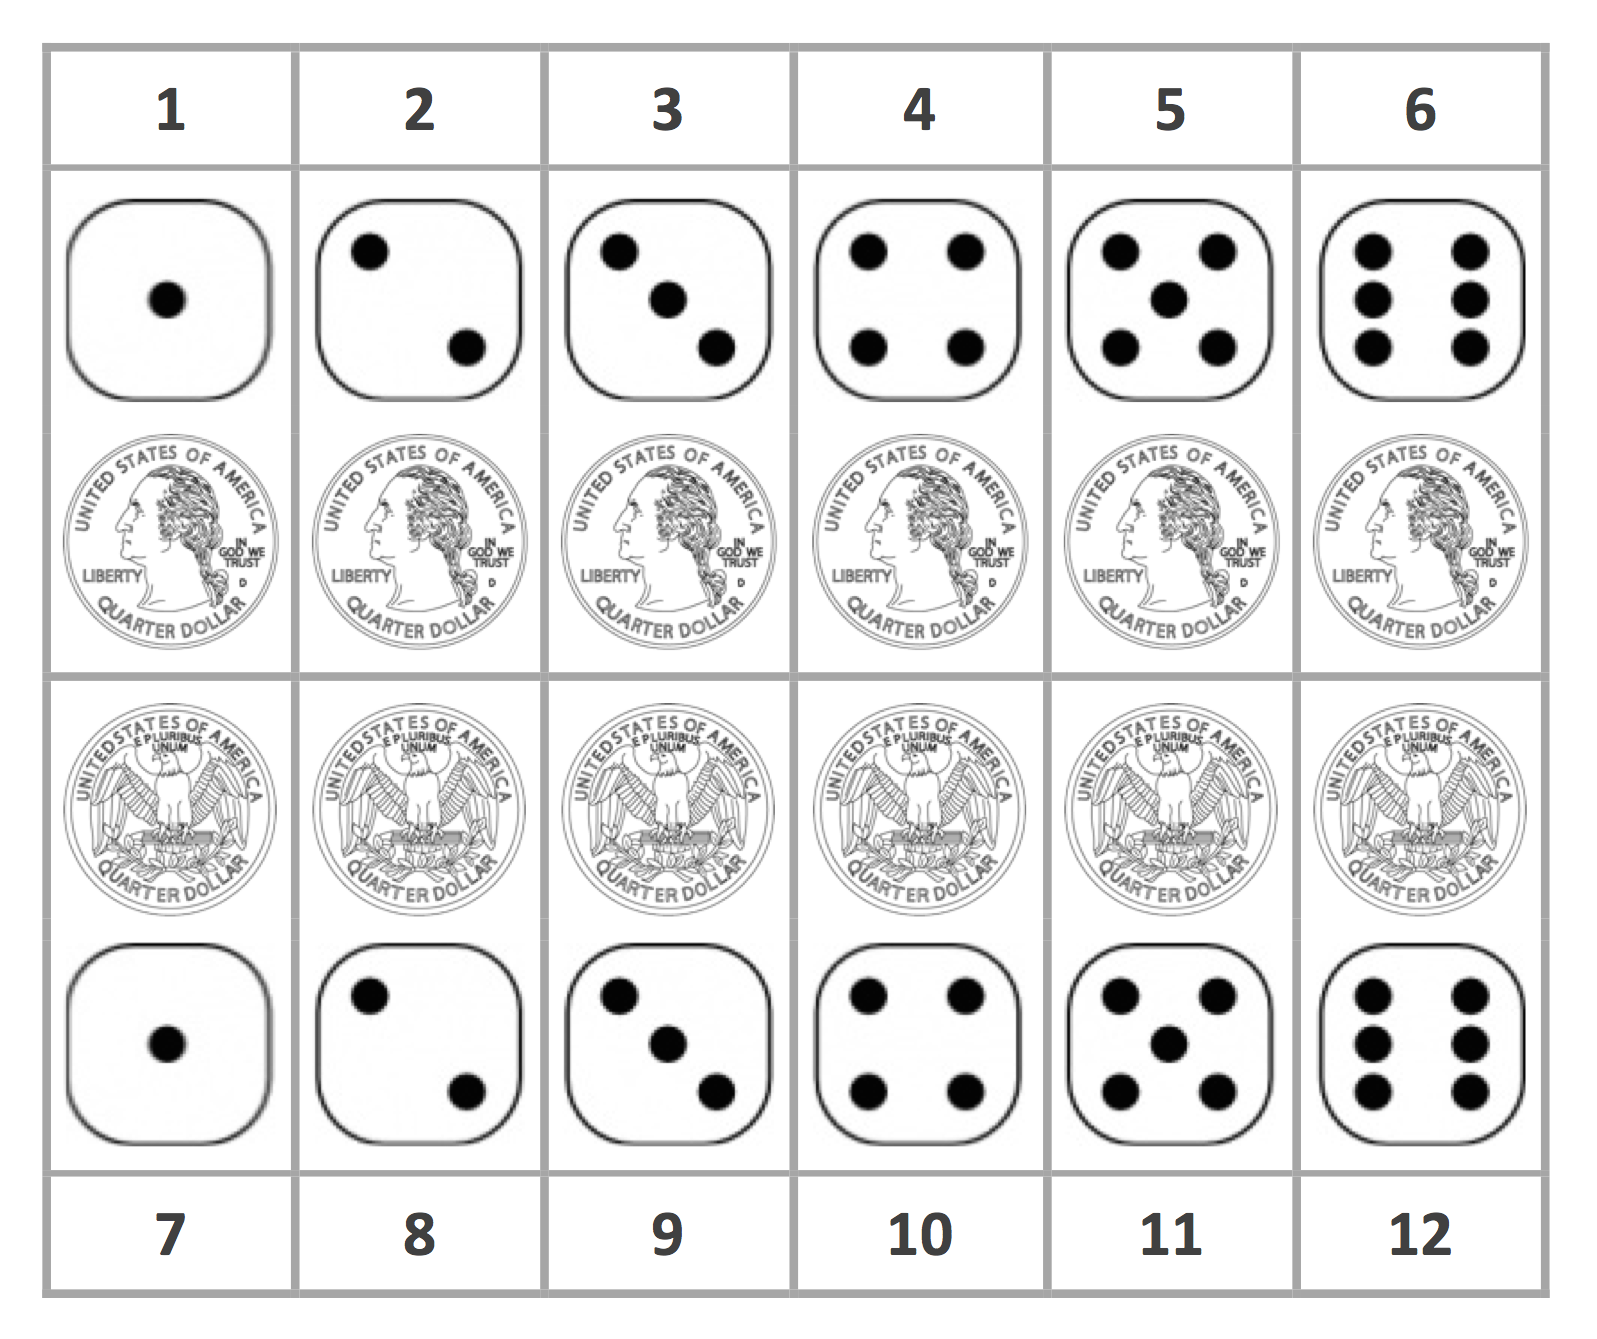
\includegraphics[width=.75\textwidth]{graphics/parameterSweep.png}
	\caption[A Scalar Parameter Sweep]{ \\ A Parameter Sweep \\ \captiontitlefinal{\textmd{over a six-sided die and a quarter.  \\ \\ Notice here that both the six-sided die and the quarter exist in a class of objects that have N distinct faces: A quarter has two faces and a six-sided die has six.  With AHAB, both these objects could be abstracted to have any multiple number of faces.} } }
	\label{fig:parameterSweep}
\end{SCfigure}
\sidecaptionvpos{figure}{b}

To get AHAB sweeping over one-dimensional vectors, though, a syntax and a construct were needed.  The syntax was needed to assist with input file parsing (see Fig.\,\ref{fig:ahabInput}), while the construct was needed to set up the logic of the sweeps (see Fig.\,\ref{fig:ahabInsert}).

AHAB's construct is how it treats variables.  This includes the distinction between: scalar and vector, completely new and old, independent values and values in sets.  Fig.\,\ref{fig:ahabInsert} shows a basic example of how this construct would handle three different variables.

The difference between the three variables in Fig.\,\ref{fig:ahabInsert} is their form of insertion.  This notion of insertion characterizes how combinations are created for the parameter sweep.  Variable (a) and variable (b) use the simpler insertions, whereas variable (c) uses a combination of the two.  

Notice in Fig.\,\ref{fig:ahabInsert} that variable (a) does not create a new combination, this is why dual insertion works: at each step of its vertical insertion process, a horizontal insertion takes place. Although the figure suggests that vertical insertion can only exist in one dimension, it can in fact take up any number of them.

\sidecaptionvpos{figure}{c}
\begin{SCfigure}[][h!]	
	\centering
	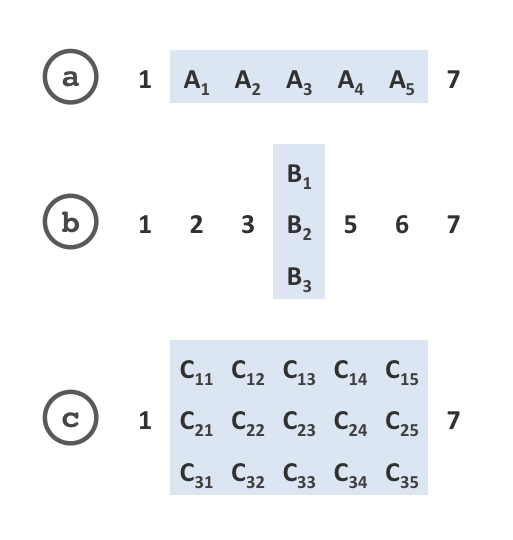
\includegraphics[width=.7\textwidth]{graphics/ahabInsert.png}
	\caption[A Vector Parameter Sweep]{ \\ A Parameter Sweep \\ \captiontitlefinal{\textmd{over three 1-D vectors. \\ \\ \textbf{(a)} uses horizontal insertion to construct large vectors. \\ \\ \textbf{(b)} uses vertical insertion to create a new vector for each value of B. \\ \\ \textbf{(c)} uses dual insertion to construct many large vectors.  It does this by using new, independent variables to combine both horizontal insertion and vertical insertion.  } } }
	\label{fig:ahabInsert}
\end{SCfigure}
\sidecaptionvpos{figure}{b}

To accomplish dual insertion, a method to add new, independent variables was needed.  In AHAB, these variables are called constants.  Fig.\,\ref{fig:ahabInput} shows how two constants, \textbf{t0} and \textbf{tDeltaFrac}, can be used to set up several vectors: \textit{tn2c}, \textit{te2c}, and \textit{tr2c}.

Fig.\,\ref{fig:ahabInput} also demonstrates several forms of syntax used by AHAB.  The \textbf{"@"} is used for constants.  The \textbf{"!"} and \textbf{"\#"} are used for comments.  The \textbf{";"} and \textbf{"|"} are used for incrementation.  And the brackets are used to distinguish vectors.  This only scratches the surface of AHAB's syntax, but gives a good overview of its use of special characters.

Lastly, notice that there are several ways to set values.  in Fig.\,\ref{fig:ahabInput}, semicolons are used to do logarithmic spacing between two values; while pipes are used to linearly increment values starting at a certain number.  This allows large lists to be constructed concisely.

\sidecaptionvpos{figure}{c}
\begin{SCfigure}[][h!]	
	\centering
	\fbox{
		\parbox{.67\linewidth}{ \texttt{
\\
\# -------------------------------------- \\
\# \ \ init ; final ; numVals  //   ( log ) \\
\# -------------------------------------- \\
\\
\phantom \ \ @t0  \ \ \ \ \ \ \ \  ! initial temperature \\
\\
\phantom \ \ \ \ \ \ \	1e-2   ;   1e+2   ;   3 \\
\\
\phantom \ \ @tDeltaFrac           !  temperature fraction \\
\\
\phantom \ \ \ \ \ \ \	100 \   ;   1000   ;   2 \\
\\
\# ---------------------------- \\
\#  \ init | increment | numVals  \\
\# ---------------------------- \\
\\
\phantom \ \ tn2c =  [ ( @t0 | @"t0/tdeltafrac" | 250 ) ] \\
\phantom \ \ te2c  \ \  [ ( @t0 | @"t0/tdeltafrac" | 250 ) ] \\
\phantom \ \ tr2c =  [ ( @t0 | @"t0/tdeltafrac" | 250 ) ] \\

		} \vspace{.15in} } 
	}
\caption[An AHAB Input File]{ \\ An Example \\ AHAB Input File \\ \captiontitlefinal{\textmd{originally used for debugging. \\ \\ Its goal was to test a new physics model for Bucky on a wide range of temperatures. This was done by setting the initial temperatures for the 250 zones' ions, electrons, and radiation. \\ \\ Here, each temperature vector would start at a value of t0 and be increased two hundred and fifty times in equal increments of t0 divided by the current value of tDeltaFrac. } } }
	\label{fig:ahabInput}
\end{SCfigure}
\sidecaptionvpos{figure}{b}







\section{Utilizing HTCondor and a Network of Computers}

As the number of combinations from parameter sweeps increases, it becomes unwieldy to run every simulation on one computer.  To remedy this problem, AHAB uses HTCondor as a method to distribute its simulations across a network of computers.  This required Bucky's start mode capabilities to be redesigned, see Appendix\,\ref{app:restart}.


\sidecaptionvpos{figure}{b}
\begin{SCfigure}[][h!]	
	\centering
	
\includegraphics[width=.72\textwidth]{graphics/HTCondor.png}
	\caption[HTCondor]{ HTCondor \\ \captiontitlefinal{\textmd{allows users to utilize a computer network's underutilized cycles.  } } }
	\label{fig:HTCondor}
\end{SCfigure}
\sidecaptionvpos{figure}{b}

HTCondor is an open-source project used for high-throughput computing (HTC).  It was created in 1984 by Miron Livny at the University of Wisconsin - Madison and was heavily developed by Michael Litzkow.  Currently, HTCondor is used at NASA, CERN, and several dozen universities \citep{htc}.   







HTCondor works by matching a user with a specific computer on their network.  Due to HTCondor's persistent motto to "leave the owner in control, regardless of the cost," matched computers are ones qualified as low-activity \citep{htc}.  On a network integrated into a computer lab, this practically means that simulations run fastest at night.

When simulations are run during peak-use times, they will frequently be lifted off busy computers and restarted on unused ones.  To allow this process to behave robustly, HTCondor offers the "Standard Universe."  This mode does, however, require a program to be compiled directly with HTCondor.  When it is difficult or impossible to do so, the "Vanilla Universe" must be used.  

Bucky uses the "Vanilla Universe" because its CMake file does not easily allow for the HTCondor compiler to be used.  In terms of development, this means that Bucky must be able to handle automatic restarts without the loss of data.  This was why the Automatic Mode was created in Bucky, see Appendix\,\ref{app:restart}.


		%\let\uppercase\relax

\vspace{24pt}

\chapter[\textbf{Conclusion}]{Conclusion}

The initial goal of this research project was to continue the work of Dr.\ Matt Terry's thesis by reconstructing his automatic tuner and then investigating target design.  Over time, however, this project has transformed into a more automation focused one, spurred on by the many common computational tasks involved in shock timing.  

This departure from creating a single-purpose automatic tuner used for investigating target design has led to many tools with relevance outside of shock ignition and even of inertial fusion. AHAB, for example, was constructed because the original automatic tuner was unsalvageable.  Although its use for this project was limited to timing the picket pulse and the pedestal pulses (see Fig.\,\ref{fig:shockConverge}), it could be used to automate the entire shock timing process.  This would increase the scope of research problems to ones requiring multiple tuned laser profiles, such as the design of fuel targets.

\sidecaptionvpos{figure}{c}
\begin{SCfigure}[][h!]	
	\centering
	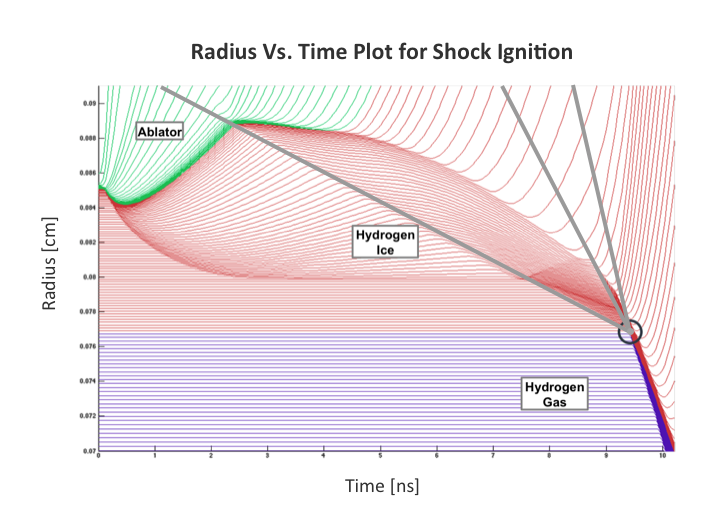
\includegraphics[width=.72\textwidth]{graphics/shockConverge.png} 
	\caption[Shock Convergence]{ The \\ Convergence of the Three Pedestal Pulses \\ \captiontitlefinal{\textmd{at the ice-gas boundary of the Hydrogen fuel source. This type of plot is discussed in Appendix\,\ref{app:rtt}.  The main point to take from it is that on a Radius Vs. Time plot, the three drawn lines represent the resulting shocks' wave speeds. } } }
	\label{fig:shockConverge}
\end{SCfigure}

In order to develop an automatic tuner, though, another program would be needed.  This program, currently codenamed Mobile Operating Batch Inspector (MOBI), would be sent to HTCondor and would then submit multiple instances of AHAB.  Further, because laser profile construction is iterative, each new laser segment could be written to its own input section, see 'Loading Multiple Input Decks from One File' in Appendix\,\ref{app:restart}.   

The first step in developing this automatic tuner would be to quantify the accuracy of shock timing.  This could be done by introducing a new parameter -- the shock breakout -- that could be inspected by MOBI in post-processing to guide future AHAB submissions.  This would prevent the need for human interpretation and interaction, both of which were used to construct the profile in Fig.\,\ref{fig:shockConverge}.

For timing the shocks, the term \textit{shock breakout} refers to when the outermost Hydrogen gas layer reaches a velocity of 3.5e5 cm/s \citep{terryThesis}.  Using this method, each new shock would have its shock breakout time plotted against its launch time.  Because a late-arriving shock would not alter this breakout time, the optimal time to start would, then, be when the breakout time just starts to move, see Fig.\,\ref{fig:shockBreakout}.

\sidecaptionvpos{figure}{c}
\begin{SCfigure}[][h!]	
	\centering
	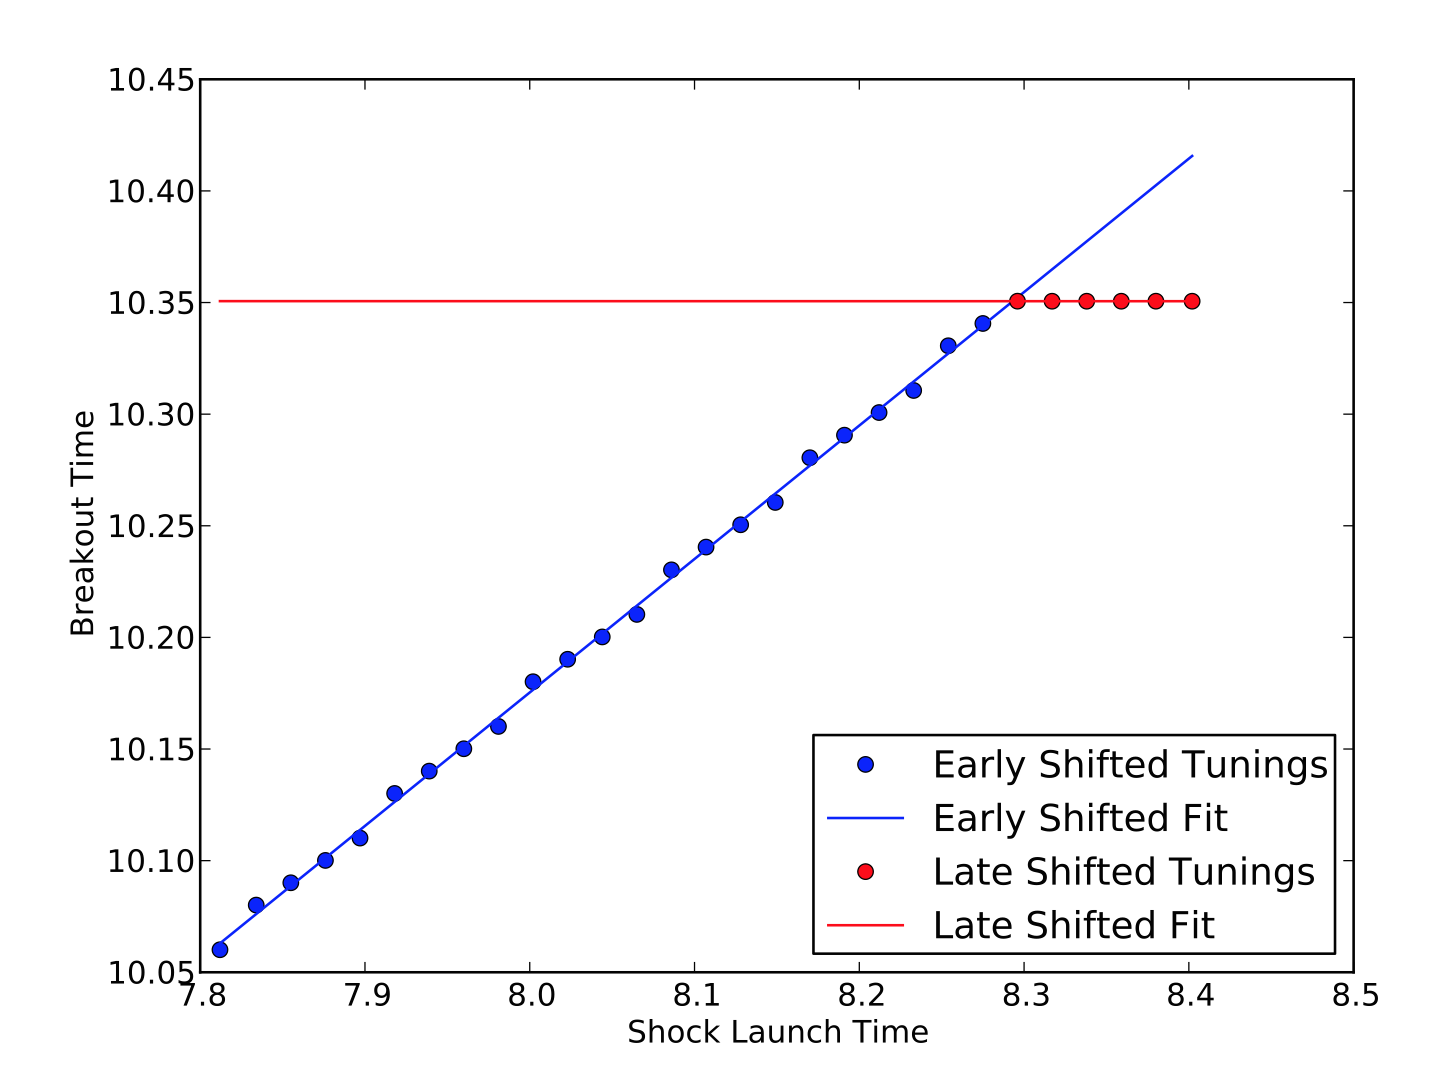
\includegraphics[width=.621\textwidth]{graphics/shockBreakout.png} 
	\caption[Automatically Timing Pedestal Pulses]{ \\ Timing a Pedestal Pulse \\ \captiontitlefinal{\textmd{requires finding the intersection between the positively sloped region of the breakout time curve and the horizontal region of it.  This is done by varying the shock launch time and measuring the resulting breakout time \citep{terryThesis}. } } }
	\label{fig:shockBreakout}
\end{SCfigure}
\sidecaptionvpos{figure}{b}

As mentioned in Sec.\,\ref{sec:mainPulses}, the compression pulse and the igniter pulse require optimizing some variable.  Although these optimized variables were stated as the target density and the energy yield, respectively, each optimized quantity could be further complicated by investigating multiple properties simultaneously.  This could include: increasing a pulse effect's robustness, achieving certain value requirements, and developing new parameters to quantize certain physical behaviors \citep{terryThesis,perkinsPaper,picketPaper}.  

Although some other unforeseen tools and analytics will be needed, AHAB should now be in a state that allows integration into a program like MOBI without too much modification.  To make sense of the Bucky output along the way, the Radius, Time, and Temperature Plot discussed in Appendix\,\ref{app:rtt} will prove to be invaluable.
		\setlength{\parindent}{\default}
	
	\endgroup
  
	\addtocontents{toc}{\protect\vspace{20pt}}

	\begin{appendices}
	
  		\setlength{\parindent}{0cm}
 		
\chapter[\textbf{The Radius, Time, and Temperature Plot}]{: \ The RTT Plotting Function}
\label{app:rtt}
The Radius, Time, and Temperature (RTT) Plotting Function is a tool used to create common plots for 1-D Lagrangian Radiation-Hydrodynamics codes, like Bucky.  The Radius and Time refer to the ordinate and the abscissa of the 2-D plot, respectively, while the Temperature is in reference to a 2-D Variable's color plot that is overlaid on top of the underlying Radius Vs. Time plot (see Fig.\,\ref{fig:basePlot}).  The Radius Vs. Time Plot is the fundamental plot for 1-D Lagrangian Codes because it represents its two computational dimensions: space, by radius, and time.

\sidecaptionvpos{figure}{c}

\begin{SCfigure}[][h!]	
	\centering
	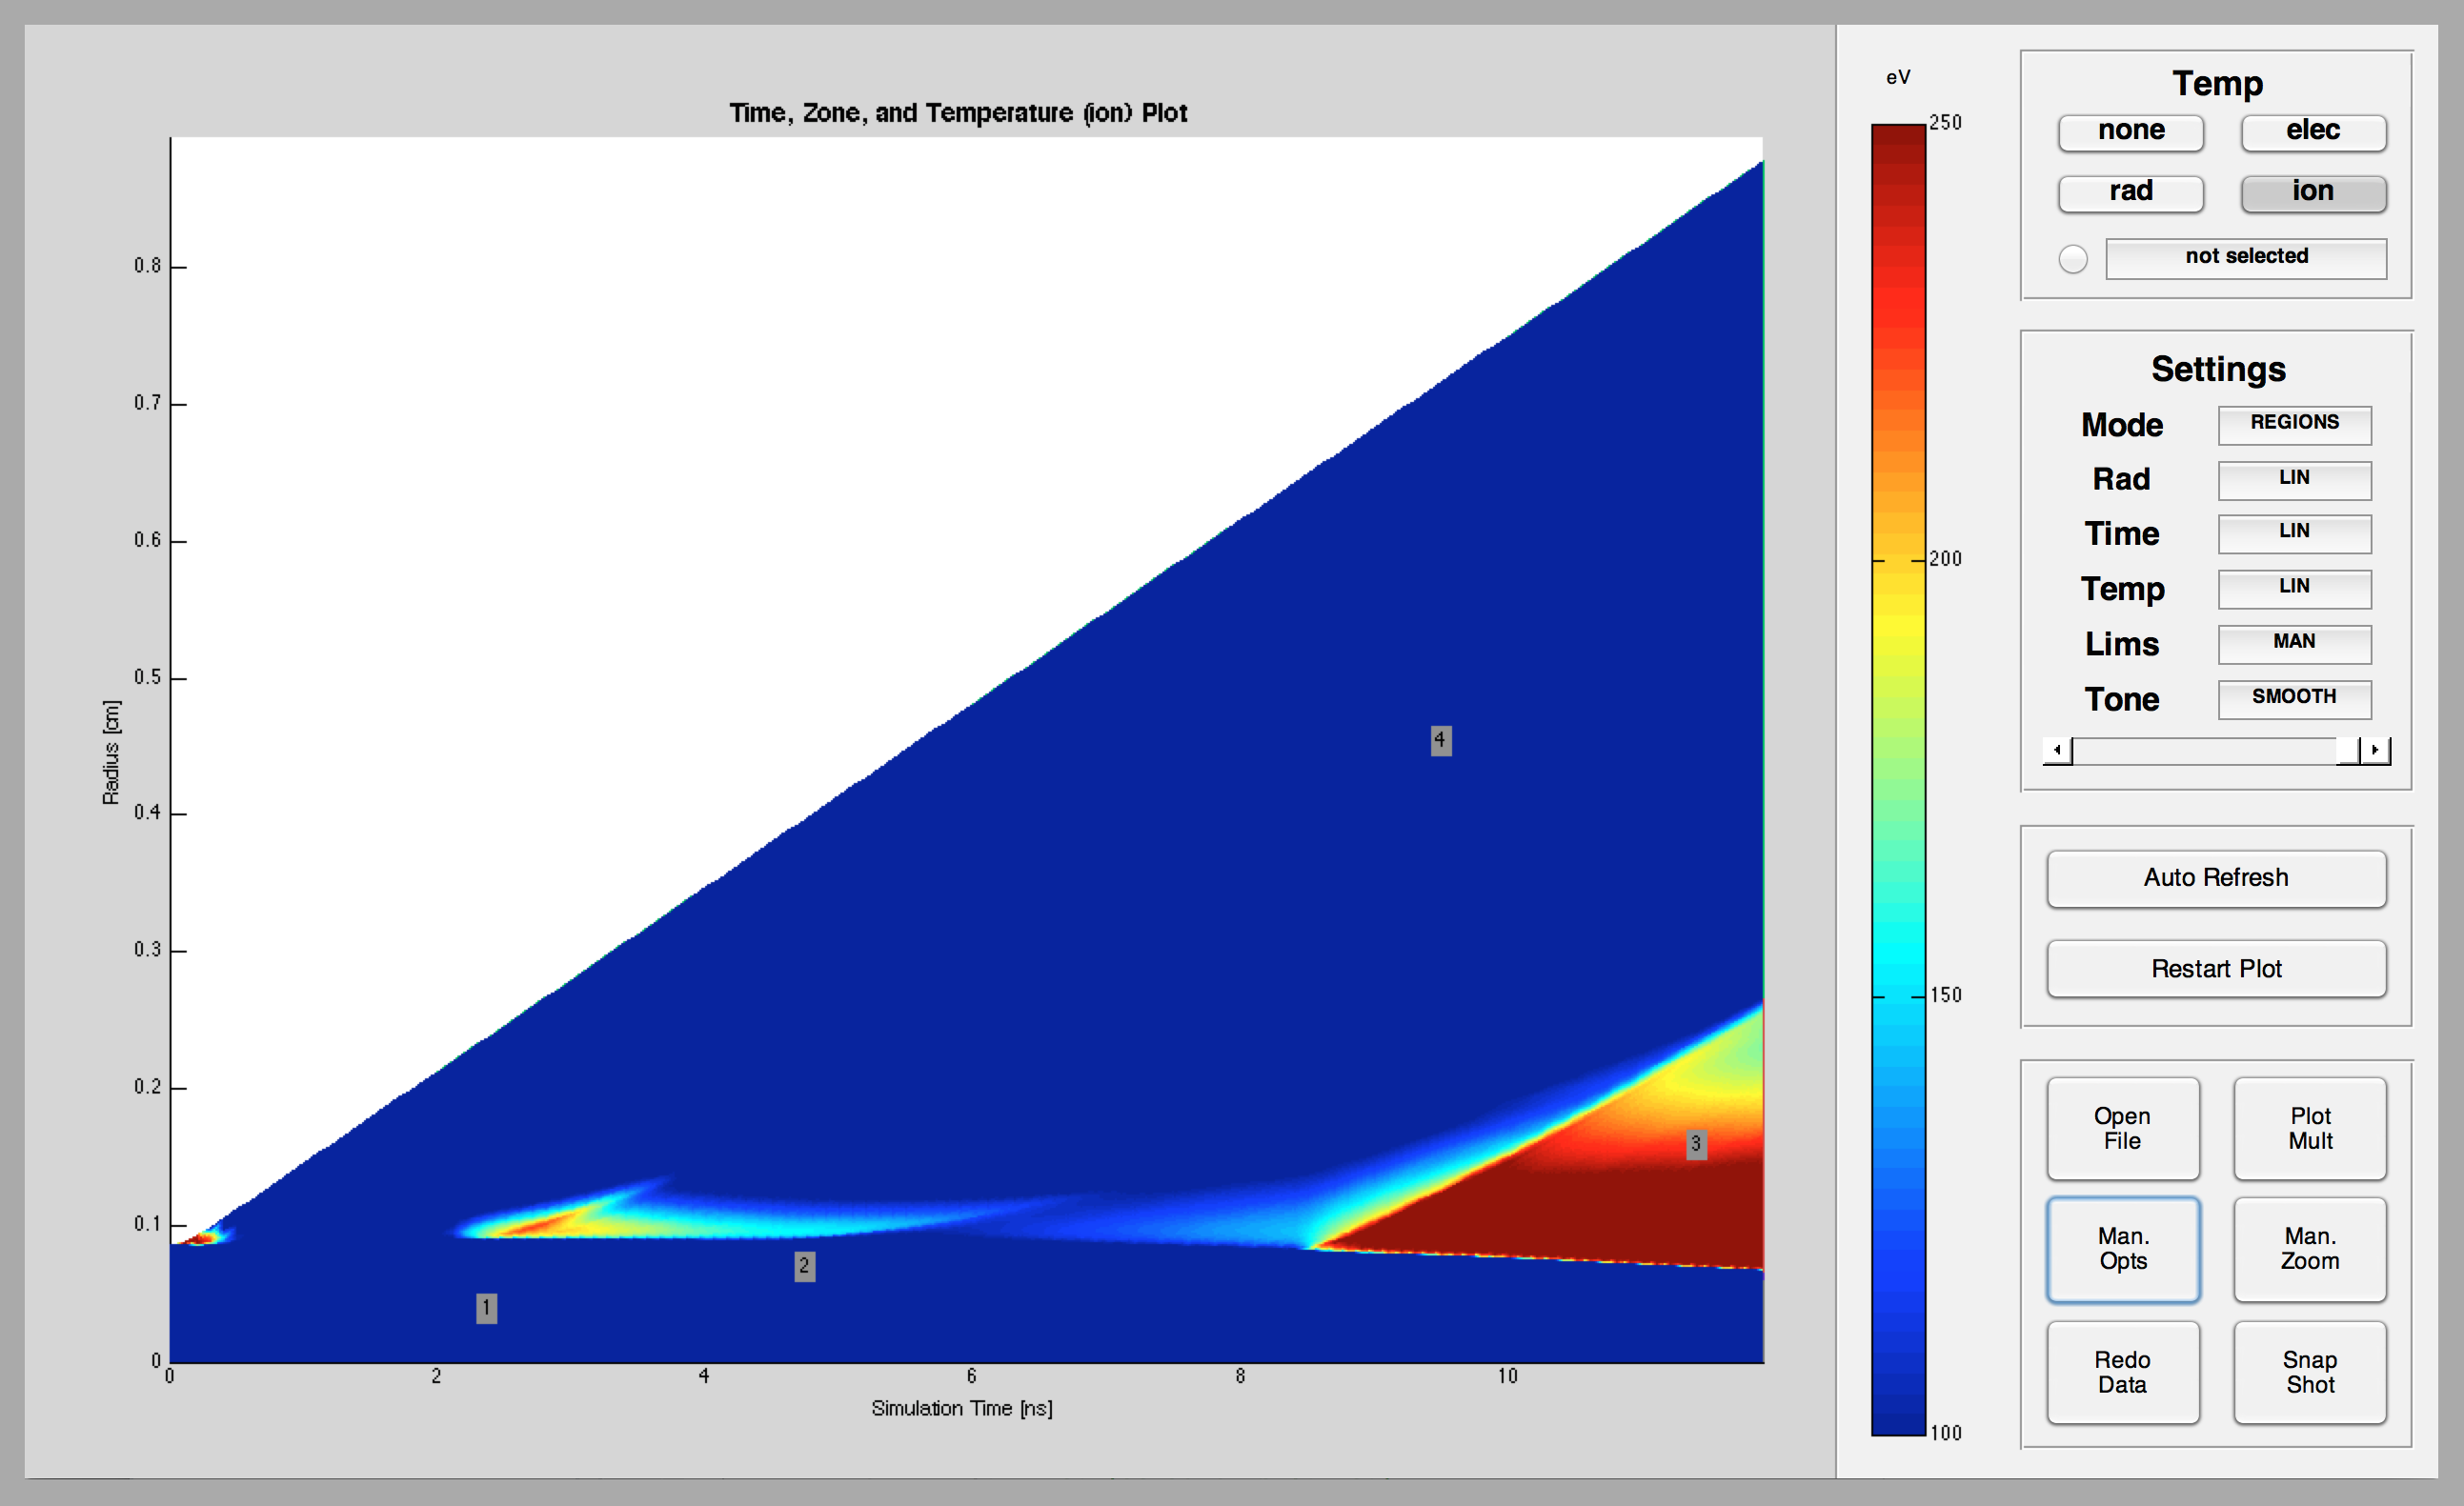
\includegraphics[scale=.23]{graphics/basePlot.png} 
	\caption[The RTT Plotting Function]{ \\ The RTT Plotting Function \\ \captiontitlefinal{\textmd{has an intricate graphical user interface that is designed to give researchers a great degree of freedom when exploring data.  The sidebar shown on the right has four sections of buttons.  The first two sections are involved in changing the plot on the left, while the bottom two deal with special utilities. } } }
	\label{fig:basePlot}
\end{SCfigure}

\subsection{A.0 \ \ Temperature Selection }

The topmost section of buttons on the GUI is involved in changing the overlaying temperature plot.  This connotation of overlaying refers to how temperature variables in Lagrangian codes have values at every spatial position and every temporal position.  

For Bucky, the three temperatures that are most relevant are: the electron temperature, the ion temperature, and the radiation temperature.  However, this notion of temperature was later redefined by extending it to include all variables that have a value for every zone and time.  This can be done by pressing the button labeled 'not selected'.

\subsection{A.1 \ \ Temperature Tone }

The bottommost button in the 'Settings' section is the Tone button.  It changes how the Temperature overlay plot is colored.  The default setting of 'Tone' is 'Smooth'.  Smooth performs an averaging scheme to its discrete data to make it look continuous.  This can prove to be dangerous in some situations because the averaging may be ill-justified.  In those situations - most commonly with logarithmic scales - it is useful to switch the 'Tone' to 'Flat'.  This mode involves no data manipulation.  

\subsection{A.2 \ \ Plot Mode }

The Plot Modes button is the first button in the 'Settings' section.  It refers to how the base Radius Vs. Time plot is done, see Fig.\,\ref{fig:comparison}.  When Mode = 'Regions', the different layers of material are colored as blocks and labeled with numbers.  When Mode = 'Lines', each Lagrangian cell boundary is plotted with region labels attached.

\begin{figure}[h!]%
\centering
\subfloat{
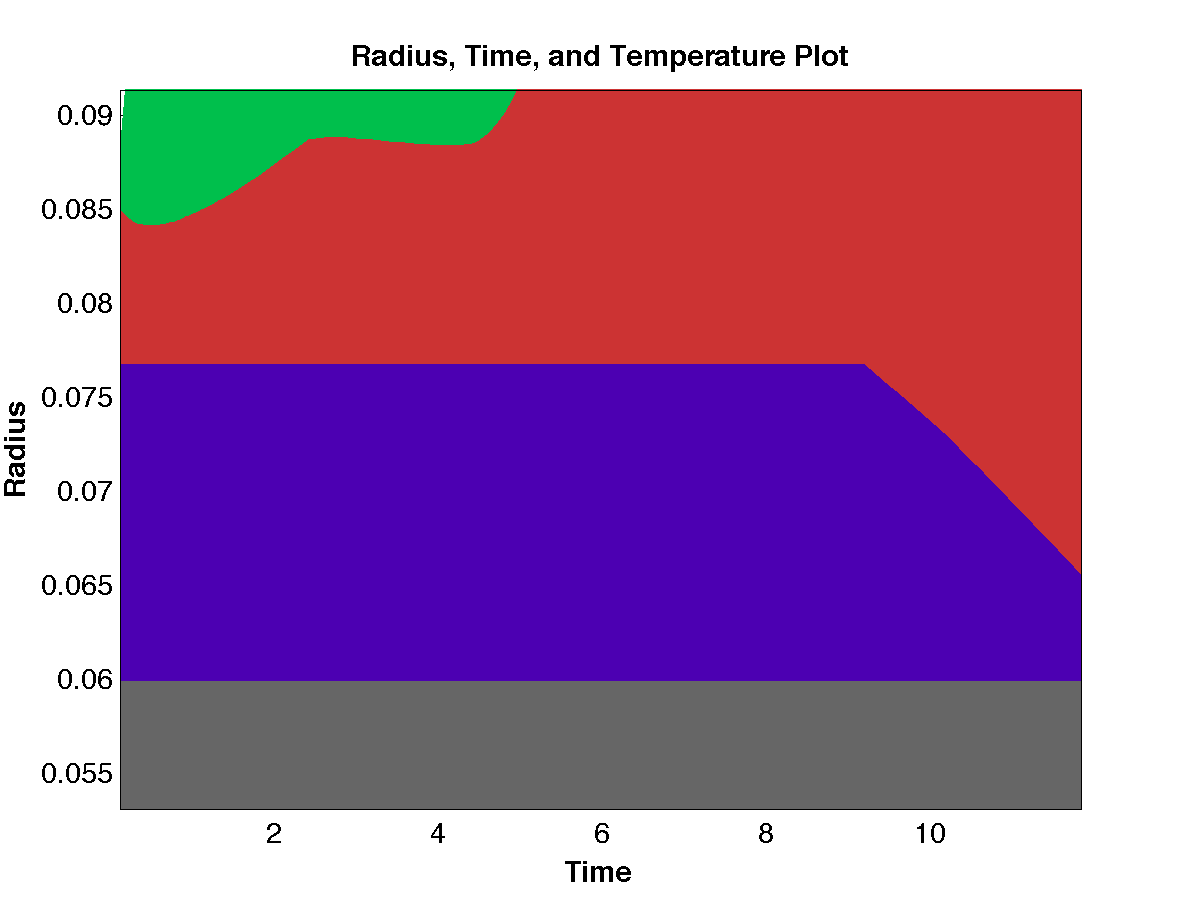
\includegraphics[width=2.5in]{graphics/regions.png} 
}\qquad %
\subfloat{
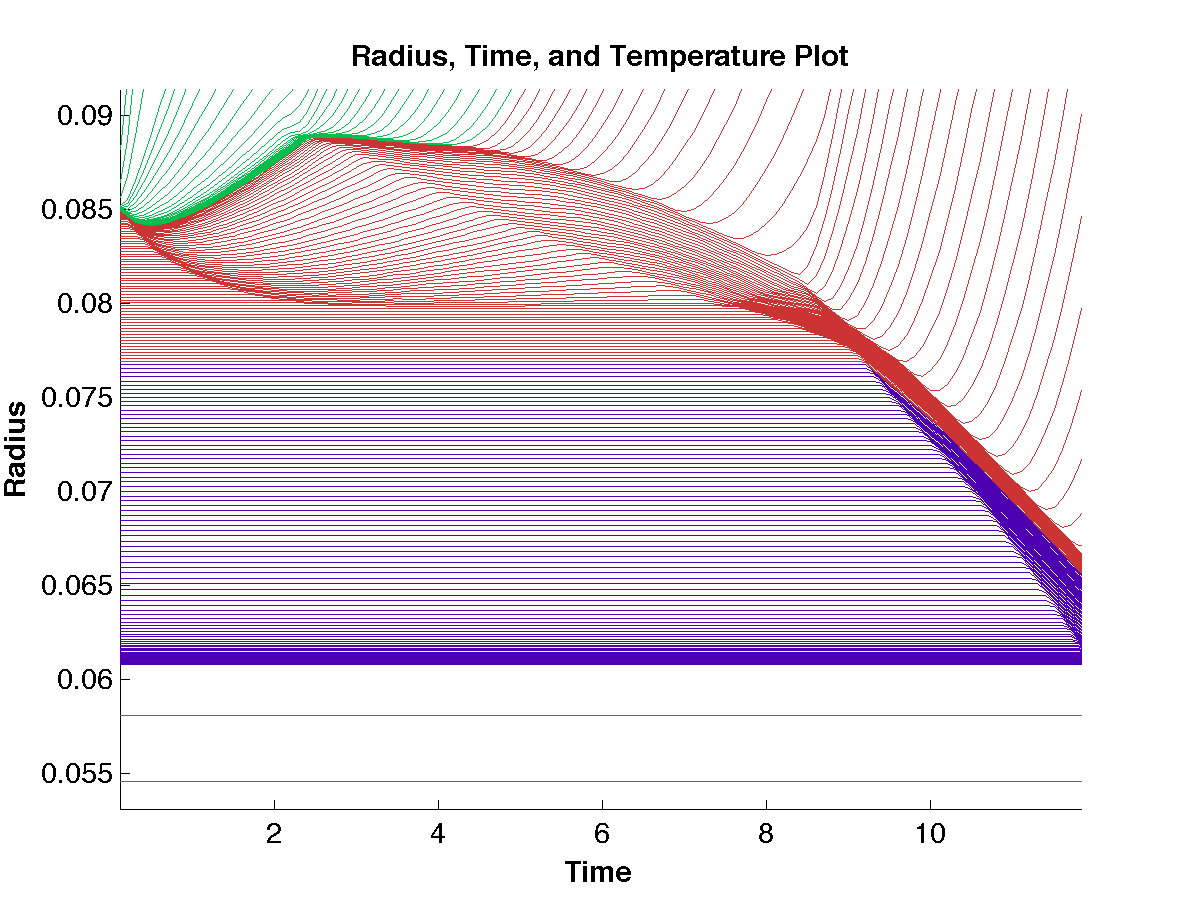
\includegraphics[width=2.5in]{graphics/lines.png} 
}
\caption[Regions Mode vs. Lines Mode]{Comparison of the Regions and Lines Plotting Modes.}
\label{fig:comparison}
\end{figure}

\subsection{A.3 \ \ Dual-Function Slider }

The Slider on the bottom of the 'Settings' section is related to the plot mode button.  When the Mode = 'Regions', the slider changes the transparency of the temperature overlay plot, where the \textit{rightmost} value is equivalent to if the base Radius Vs. Time Plot is completely hidden and the \textit{leftmost} value is equivalent to if 'none' is selected in the 'Temp.' section. When the Mode = 'Lines', the slider changes the number of zone boundary lines that get shown.

\subsection{A.4 \ \ Scales }

The RTT function has three buttons in the 'Settings' section that change the scaling of the problem.  Initially, all three scales - radius, time, and temperature - are set to linear.  They can each be changed to logarithmic and back by clicking their respective buttons.

\subsection{A.5 \ \ Manual Limits }

In addition to changing the scaling of the problem, another common plotting problem is imposing certain limits (i.e. maxima and minima).  This can be done for the radius, the time, and the temperature; however, the temperature is handled differently.  

\begin{wrapfigure}{r}{0.38\textwidth} %[][h!]	
	\vspace{-24pt}
	\centering
	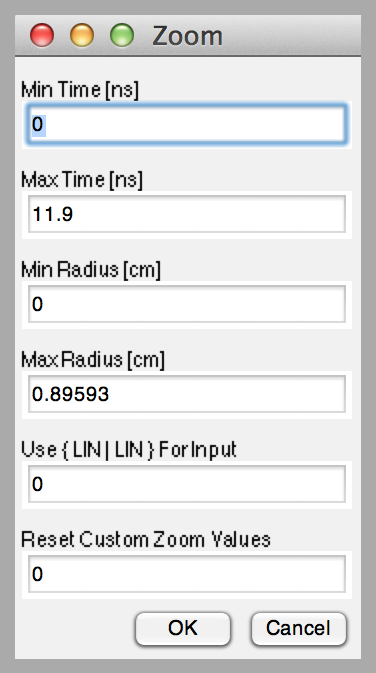
\includegraphics[scale=.83]{graphics/manZoom.png} 
	\vspace{-4pt}
	\caption[Manual Zoom Input Box]{ \small{The Zoom Input Box }\\ \captiontitlefinal{\small{\textmd{gives users a way to zoom to specific areas of the plot. Changing "Lin|Lin" forces these values to be linear, while changing "Reset 'Custom Zoom Values" resets them. } }} }
	\label{fig:manZoom}
\end{wrapfigure}

The Temperature limits involves two buttons that are combined for the other variables.  The first button is \mbox{'Man. Opts'}, which changes the maximum and minimum temperature, while the second button is 'Lims' in the 'Settings' section.  Initially, the 'Lims' button is set to 'Auto', but can be changed to 'Manual'.  The 'Manual' setting changes the temperature limits from the automatically chosen ones to the values inputted in \mbox{'Man. Opts'}.  By default, these limits are 0.1 eV and 200 eV.

For Radius and Time, the manual limits are controlled with the 'Man. Zoom' button.  The term manual refers to how it differs from the automatic zoom that is imposed on the plot at the beginning of the program.  Manual zooming is, thus, changing the minimum and maximum values for the radius and for the time.  With the input box, this can be done in both the current scale and the Linear-Linear scale.  Additionally, the input box allows a way to restart the extrema to their initial values, which are in turn set by the current file's data, see Fig.\,\ref{fig:manZoom}.

\subsection{A.6 \ \ Loading and Reloading Data }

Several buttons in the bottom two sections provide loading and reloading functionality.  'Open File' opens a prompt for users to select a new file to load.  This function is called at the beginning of the RTT function, either implicitly if a data file exists in the local directory, or explicitly with a prompt if no data file is found.  

The 'Redo Data' and the 'Auto Refresh' buttons offer two ways to reload data.  The 'Redo Data' button reopens the current data file.  This is useful for when a run is restarted.  The 'Auto Refresh' reopens the current data file 'n' times at regular intervals of 'm' seconds.  This is useful for when the RTT plot is being used while a Bucky simulation is simultaneously running.  The values of 'n' and 'm' are set inside 'Man. Opts' with default values of 10 seconds and 500 times, respectively.

The 'Restart Plot' button is used to return every selection in the top three sections to their original values. It is located inside the same section as  'Auto Refresh' because it is the only button able to turn off the 'Auto Refresh' effect -- besides by pressing of the \mbox{'Auto Refresh'} button again.  


\subsection{A.7 \ \ Saving the Current Plot to a File }

The 'Snap Shot' button allows researchers to save the current plot to an image.  This is commonly needed for published documents and presentation slides.  This routine has a user select a file name, a destination, and an image type and then saves the plot there.  This function most notably increases the font sizes and removes the background color. 


\subsection{A.8 \ \ Plotting Multiple Files }

The 'Plot Mult' button allows users to open a whole directory of data files and displays their contents inside a scrollable window, see Fig.\,\ref{fig:plotMult}.  The plots produced by this will all share the options set by the user in the top two button sections of the main plot.  

Additionally, when the directory is created by AHAB, every plot's zoom feature is connected together.  This allows users to see the subtle differences in their data (e.g. the arrival time of a specific shock at a certain zone). 

\begin{figure}[h!]	
	\centering
	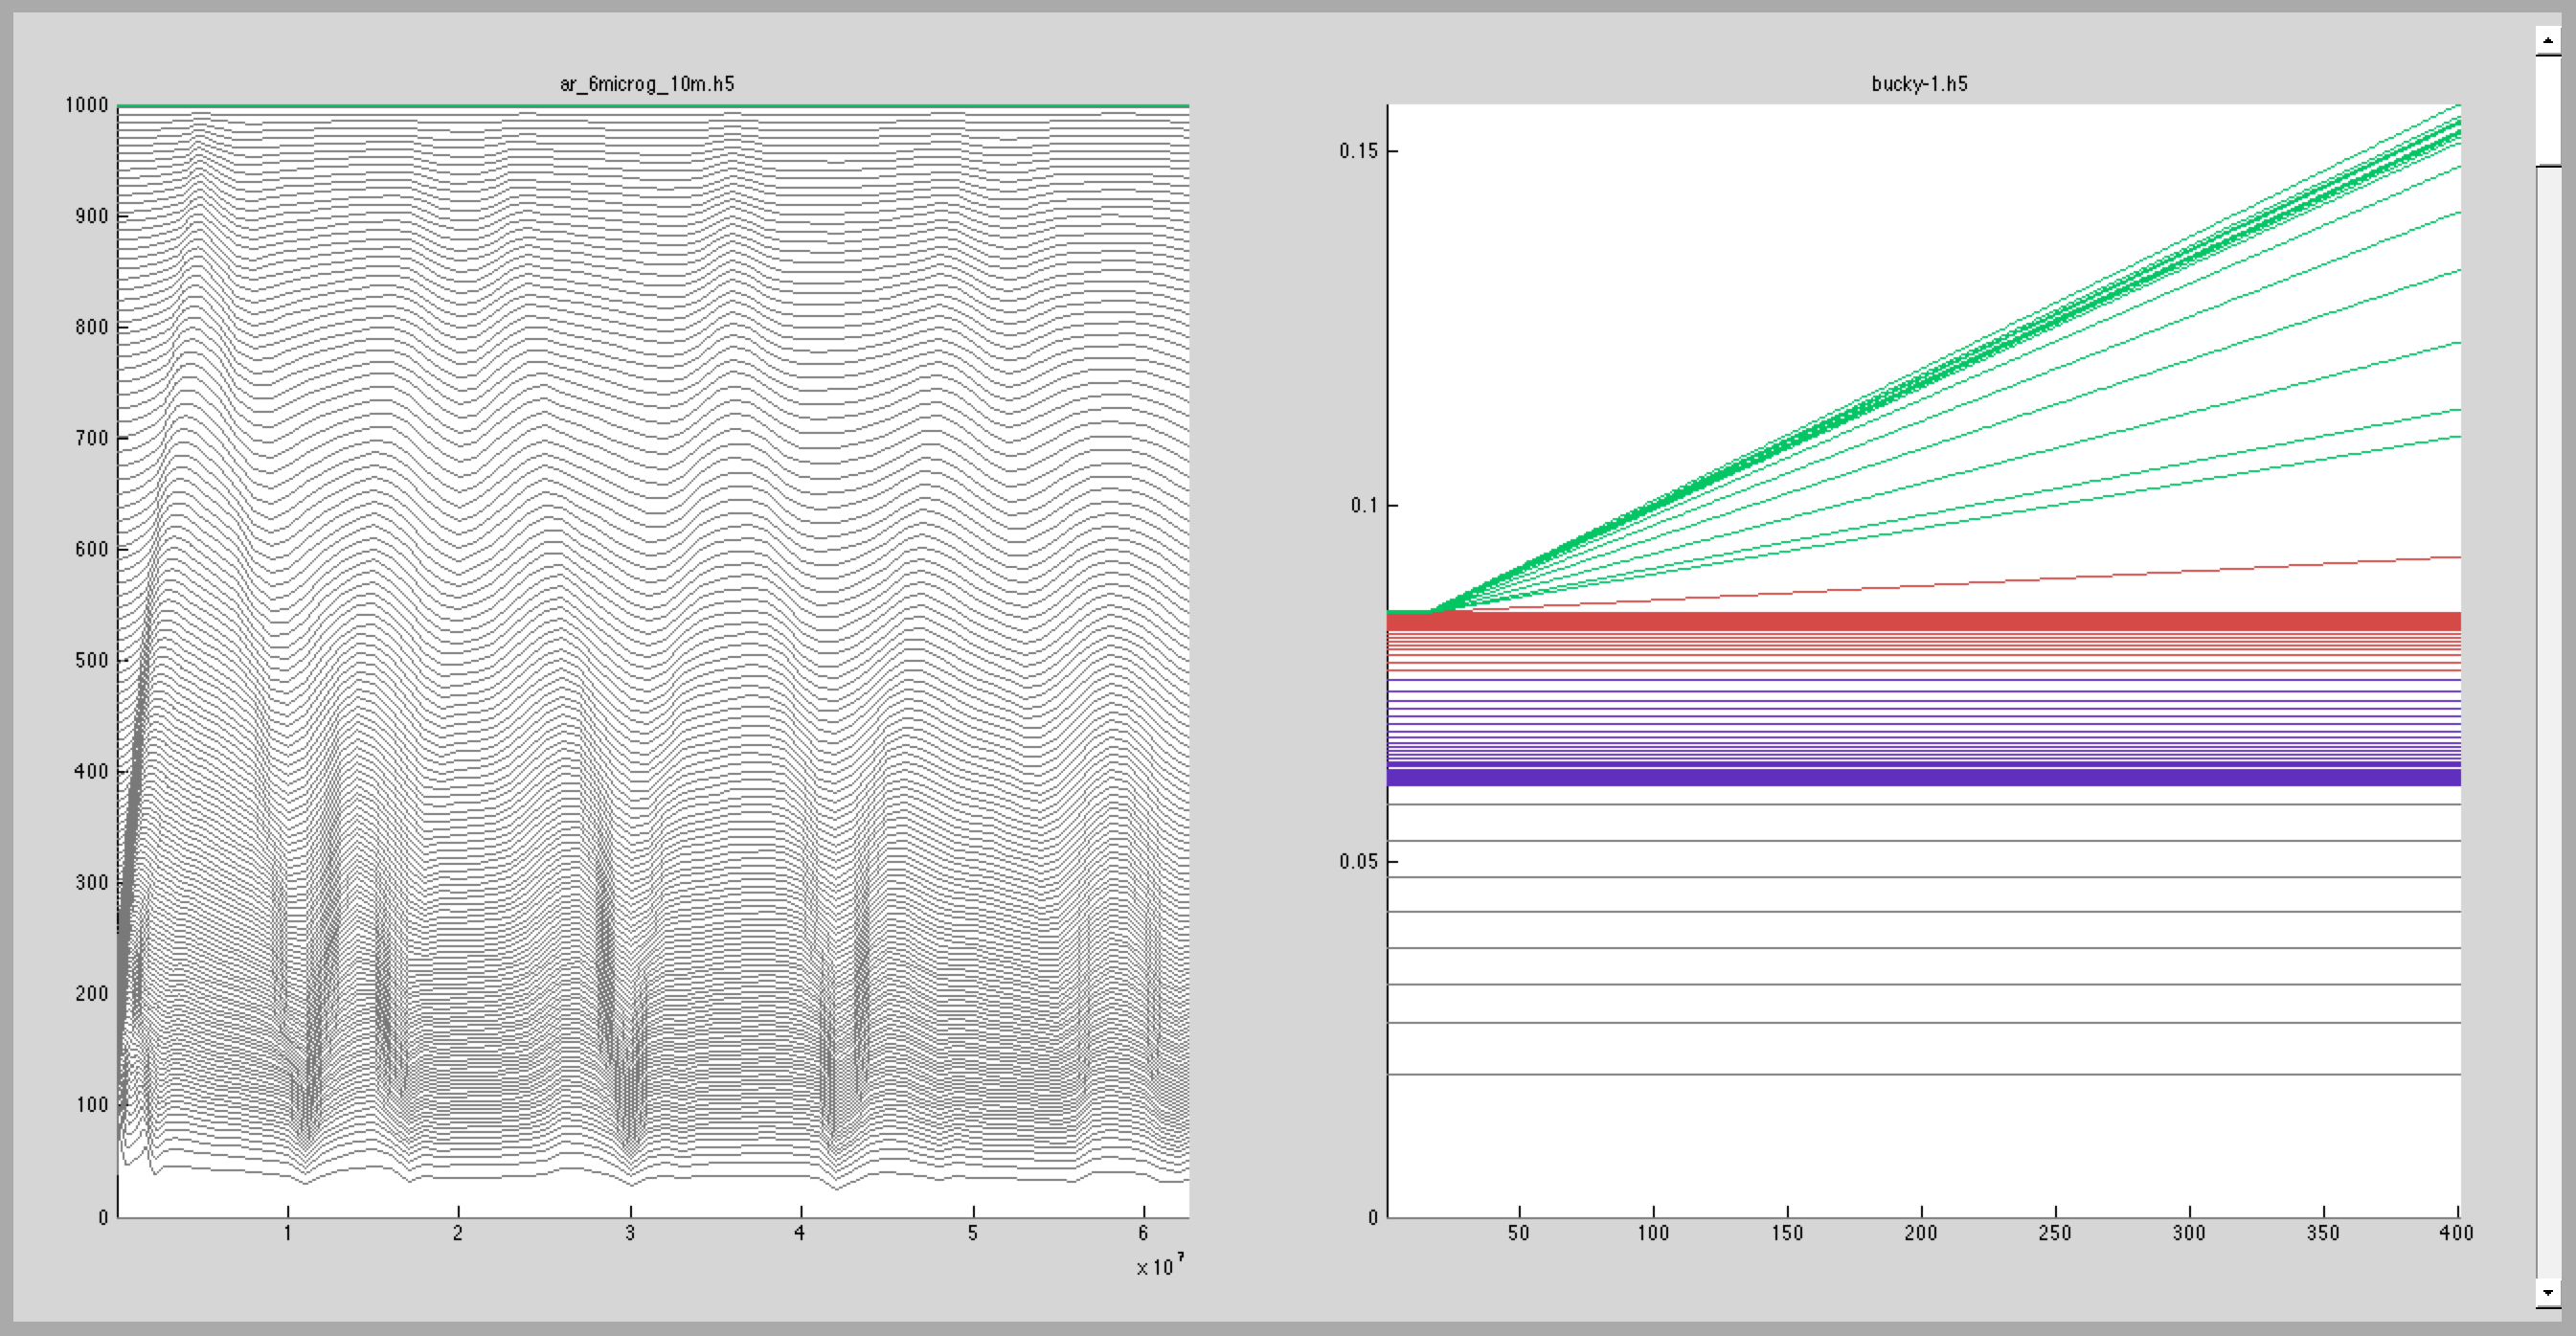
\includegraphics[width=0.68\textwidth]{graphics/plotMult.png} 
	\caption[Plotting Multiple Files]{  The 'Plot Mult' Button \\ \textmd{plots multiple files inside one window. \\ } \tiny{\phantom \\ \phantom} } 
	\label{fig:plotMult}
\end{figure}

\subsection{A.9 \ \ Adding Points to the Plot }

The last feature the RTT plot offers is the "Points Layer."  In the RTT plotting function, each plot is given its own layer (i.e. the Radius Vs. Time Layer, the Temperature Layer, the Text Layer).  The Points Layer is another layer that allows users to add points to the current plot.  These points transform under scale transformations and zooming.  

Additionally, while hovering over the plot in the GUI, a crosshairs is generated; this crosshairs is composed of a vertical line and horizontal line that meet at the cursor and extend to the boundaries of the plot.  When any key besides 'Delete' or 'Escape' is pressed without a modifier (i.e. 'Shift'), a point appears on the plot and has its linear scale coordinates entered on the top left of the screen.  Any number of points can be added to the plot; however, they are all removed when opening a different file. 

\sidecaptionvpos{figure}{b}

\begin{SCfigure}[][h!]	
	\centering
	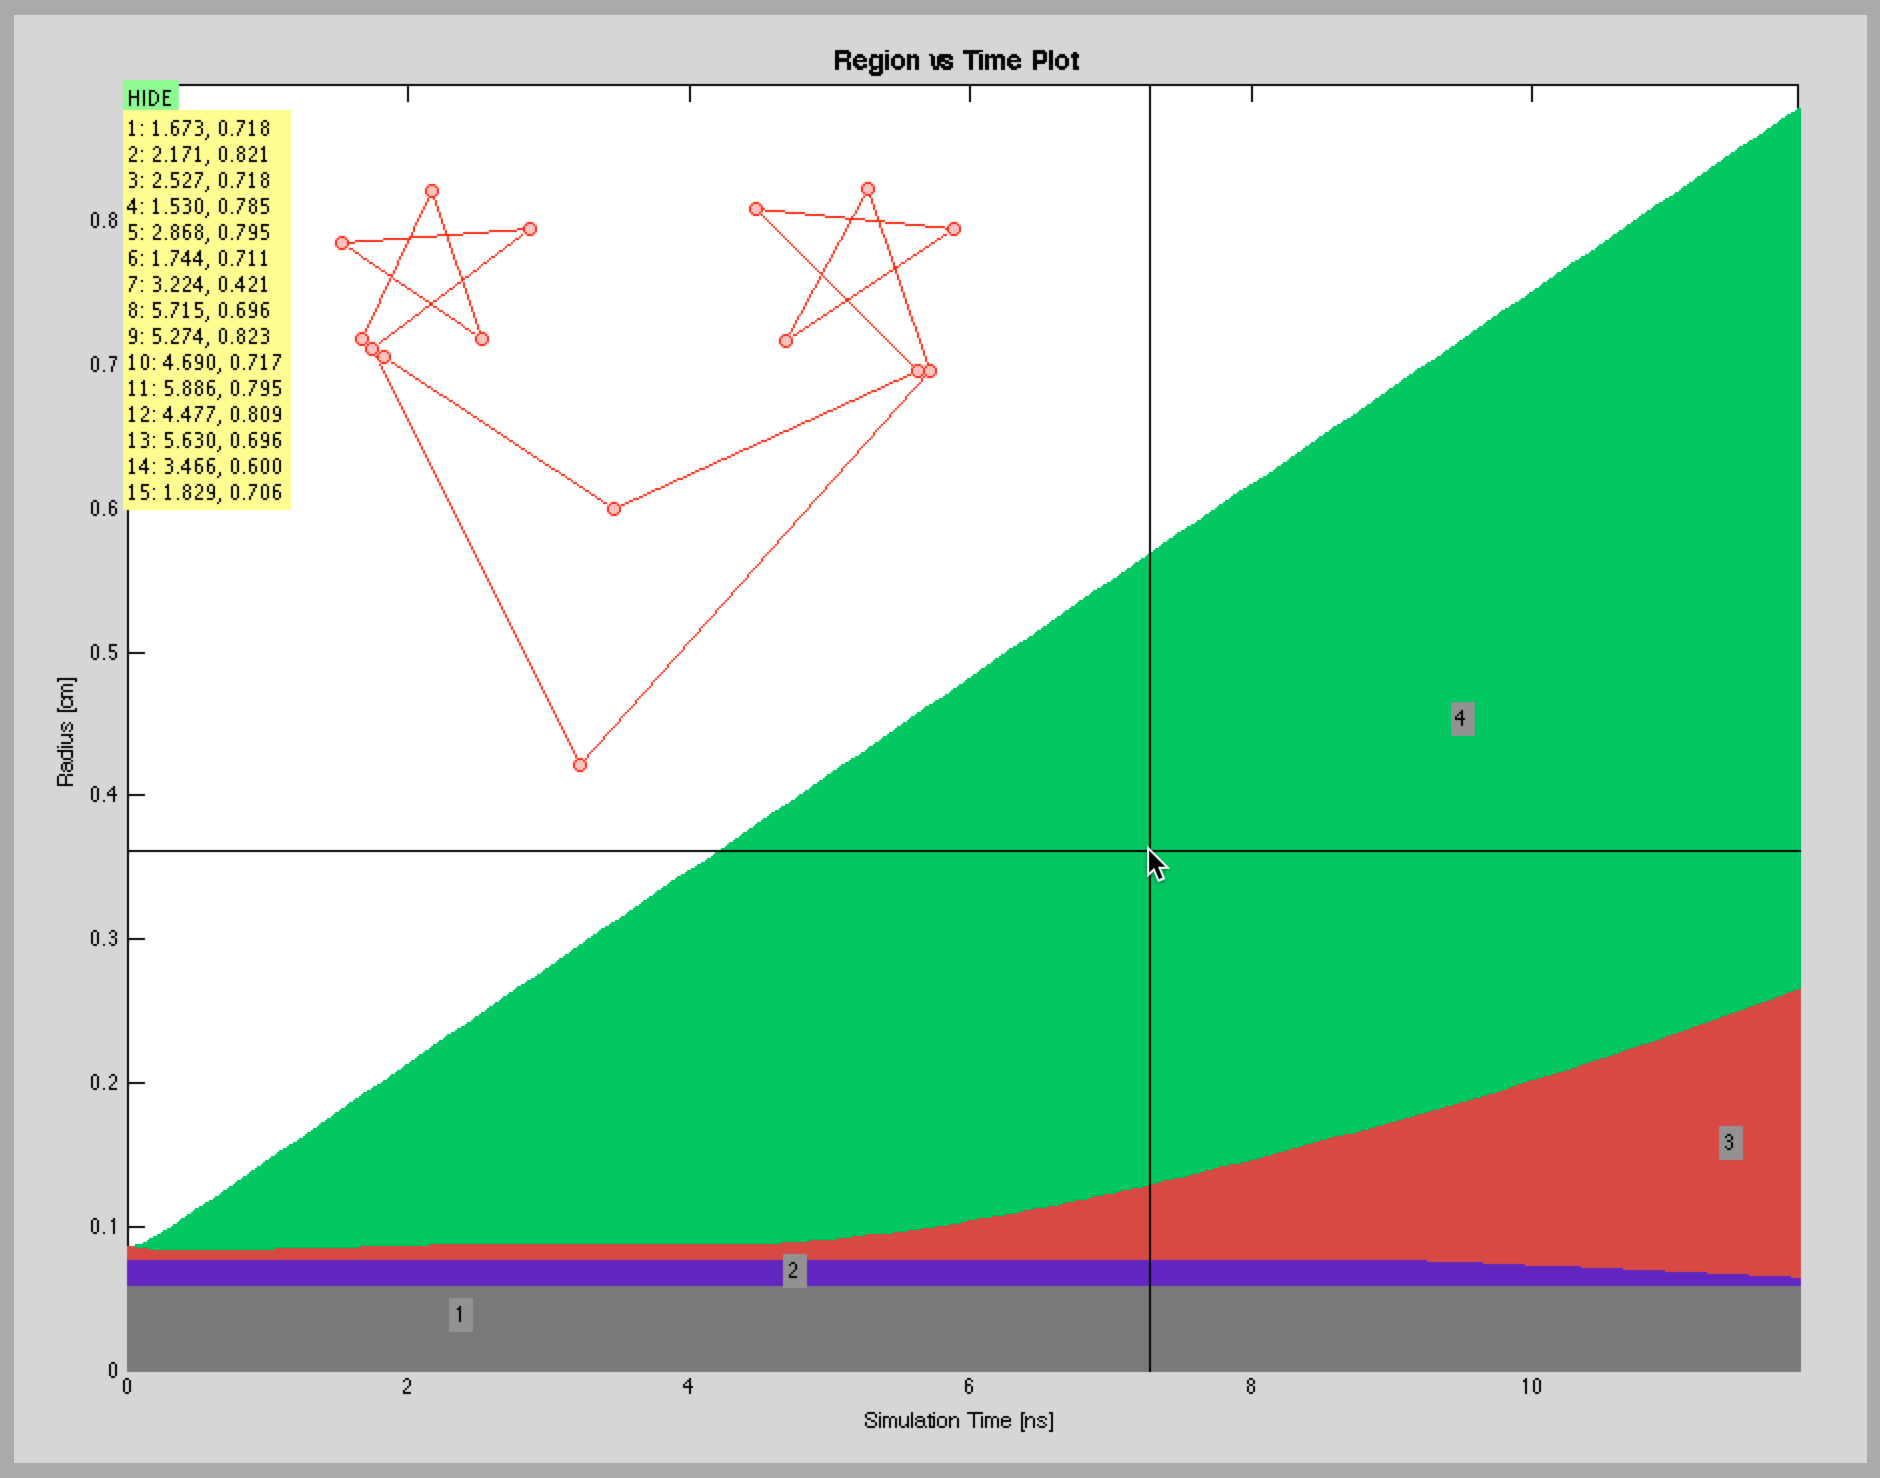
\includegraphics[scale=.24]{graphics/pointsLayer.png} 
	\caption[The Points Layer]{ \\ The Points Layer \\ \captiontitlefinal{\small{\textmd{allows points to be added to the current plot.  This is done by pressing most keyboard keys while hovering over the plot. These points persist through scale changes, but are removed when the file is changed. The coordinates are displayed in the top-left of the plot. } } }}
	\label{fig:pointsLayer}
\end{SCfigure}

  		
\chapter[\textbf{Bucky Start Mode Capabilities}]{: \ Bucky Start Mode Capabilities}
\label{app:restart}
The Bucky start mode capabilities allow users to stop and restart simulations at whim. This allows minor changes to be made to the code or the input file without the need for repeating the whole simulation. This functionality is controlled by the user using the two namelist restart variables: \textbf{mstart} and \textbf{ncycrs}, which specify the start mode and the cycle number, respectively (see Fig.\,\ref{fig:bucky.inp}).

\sidecaptionvpos{figure}{c}

\begin{SCfigure}[][h!]	

	\centering
	\fbox{
		\parbox{.4\linewidth}{ \texttt{
			\\
			\$rstart  \\ 
			\phantom \ \ \ \ \ \ \ \ \ mstart \ = \ 2  \newline
			\phantom \ \ \ \ \ \ \ \ \ ncycrs \ = \ 200  \\
			\$end \\
			\\ 
			\$input \\
			\phantom \ \ \ \ \ \ \ \ \ nmax \ \ \ = \ 1300 \\
			\phantom \ \ \ \ \ \ \ \ \ tmax \ \ \ = \ 5.0E-09 \\
			\phantom \ \ \ \ \ \ \ \ \ iorest \ = \ 500 \\
 			\$end
		} \vspace{.15in} } 
	}

\caption[A Bucky Input File]{ \\ Example 'bucky.inp' File \\ \captiontitlefinal{\textmd{that shows the common structure for using the start mode functionality.  \\ \\ Inside the \textbf{\$rstart...end\$} block, \\ mstart and ncycrs are changed.  \\ Inside the \textbf{\$input...end\$} block, below that, every other variable is changed.* \\ \\ \small{*\,For this specific example, the input deck is short because it is for a restart run that does not need to specify the initial conditions of the problem. } } } }
	\label{fig:bucky.inp}
\end{SCfigure}

\sidecaptionvpos{figure}{b}

\subsection{\texttt{[ 0]} \ -- \ Standard Mode}

In Standard Mode, when mstart = 0, the current simulation is treated as an initial run.  This means that it will overwrite output files, e.g. bucky.h5 and bucky.out.  It also means that the code treats its input file as if it had no restart block at all.

\subsection{\texttt{[ 1]} \ -- \ Restart Mode }

In Restart Mode, when mstart = 1, the current simulation starts from a cycle found in the restart logs of either \textbf{bucky.cur\_restart} or \textbf{bucky.new\_restart}.  Restart logs are created at every \textbf{\textit{iorest}} cycles when the code is in either the standard mode or the restart mode.

\pagebreak

The cycle that the restart mode loads from is the closest one to \textbf{ncycrs} in either bucky.cur\_restart or bucky.new\_restart.  This means that if ncycrs is greater than or equal to the first log in bucky.cur\_restart, the algorithm chooses the closest cycle in either of the two files and loads from it.  Additionally, if ncycrs is less than or equal to zero, the code short-circuits to loading the newest log in bucky.new\_restart.

When starting a new restart, two things are done.  First, if the current log was found in bucky.new\_restart, bucky.new\_restart is relinked as bucky.cur\_restart before being read. Second, the base names of the output files are changed to reflect an advancement in restart number.  For example, after the initial run, the first restart changes the text output file from bucky.out to bucky1.out; on the second restart, the text output file changes from bucky1.out to bucky2.out.

\subsection{\texttt{[ 2]} \ -- \ Automatic Mode  }

In Automatic Mode, when mstart = 2, a simulation is allowed to efficiently advance to completion, even in the face of frequent and unprompted restarts.  This mode was originally designed for HTCondor's vanilla version, which is discussed in Section 4.2.  The main difference between Restart Mode and Automatic Mode is that Restart Mode has files filled with restart logs written every iorest cycles, while Automatic Mode uses checkpoints updated every iorest cycles.  

This difference in nomenclature stems from the fact that checkpoint files only have one restart log a piece.  Bucky therefore keeps three checkpoint files in Automatic Mode: a backup file with the initial conditions of the simulation set (bucky.restart\_0) and two leapfrog files that have their logs updated every other time (bucky.restart\_1 and bucky.restart\_2).  Additionally, if bucky.restart\_0 has either been corrupted or deleted, a simulation in this mode will start over from the beginning.  

\subsection{\texttt{[10]} \ -- \ Merge Mode  }

In Merge Mode, when mstart = 10, Bucky merges all the output files made by Restart Mode into the main output files (up to the \textbf{ncycrs} cycle or to the most recent cycle if specified, otherwise).  This means that \mbox{bucky1.h5 , \ldots \ , buckyN.h5} as well as \mbox{bucky1.out , \ldots \ , buckyN.out} are merged into bucky.h5 and bucky.out , respectively. 

After this mode, the restart logs are wiped and an updated restart file is made in their place.  This is why Automatic Mode calls it after it has completed its simulation.  Automatic Mode does not back up its files like Restart Mode does because it has no way to go back more than two checkpoint logs ago, rendering labeled output files useless.

\subsection{Loading Multiple Input Decks from One File }

Bucky also has the capability of loading multiple input decks from within one file.  This is useful because it removes the need to either use multiple input files or edit a single file, both of which are extremely prone to human error.  The multiple input deck capability also gives many different spots to restart a simulation, as long as it was not merged along the way.

When there are multiple input decks in one file, they are read sequentially. However, if the first deck is in Standard Mode or in Automatic Mode, it must be kept at the bottom.  This is because these decks contain the initial conditions of the problem and are consequently much longer.  After this first read, though, the input pointer returns to the top of the file and works its way down.

For runs \underline{not} taking advantage of the Automatic Mode, using multiple input decks in one file behaves as if there were N input files read one at a time.  This means that mstart can only be equal to: 0, 1, and 10.  This protocol refers to having one Standard Mode Run, followed by any number of Restarts and Merges given in any order.

When Automatic Mode is used with multiple input decks, restarts can take advanced savings in storage space, speed, and human error.  This is increasingly true for longer simulations and larger input files where early cycles become decreasingly important. 

To use Automatic Mode with multiple input decks, set all input decks that are no longer the focus of interest to Automatic Mode.  This must include the initial Standard Mode run and continue until the first Restart Mode.  It is important to note that after transitioning from Automatic Mode to Restarts and Merges, there is no going back.  For this mode, mstart can only be equal to: 2, 1, and 10.
 		\setlength{\parindent}{\default}
 		
 	\end{appendices}

	\include{backmatter/backmatter}
	\backmatter

	\bibliographystyle{IEEEtran}
	\bibliography{IEEEabrv,references}

\end{document}


\pagebreak
\vspace*{\fill}
\vspace{-32pt}
\centering{
	\large{
	\bf{
		\texttt{
			This page intentionally left blank.
}}}}
\vspace*{\fill}

